%
% Tesi D.S.I. - modello preso da
% Stanford University PhD thesis style -- modifications to the report style
%
%%%%%%%%%%%%%%%%%%%%%%%%%%%%%%%%%%%%%%%%%%%%%%%%%%%%%%%%%%%%%%%%%%%%%%%%%%%
%                                                                         %
%			TESI DOTTORATO                                                   %
%			______________                                                   %
%                                                                         %
%			AUTORE: Elena Pagani                                             %
%                                                                         %
%			Ultima revisione: 7.X.1998                                       %
%           correzioni atrent                                             %
%%%%%%%%%%%%%%%%%%%%%%%%%%%%%%%%%%%%%%%%%%%%%%%%%%%%%%%%%%%%%%%%%%%%%%%%%%%
%
%
\documentclass[a4paper,12pt]{report}
%    \renewcommand{\baselinestretch}{1.6}      % interline spacing
%
% \includeonly{}
%
%			PREAMBOLO
%
\usepackage[a4paper]{geometry}
\usepackage[italian]{babel}
\usepackage{amssymb,amsmath,amsthm}
\usepackage{graphicx}
\usepackage{url}
\usepackage{hyperref}
\usepackage{epsfig}
\usepackage{setspace}
\usepackage{tesi}
\usepackage{amssymb}
\usepackage{amsmath}
\usepackage{hyperref}
\usepackage{color,soul}
\usepackage{float}
\usepackage{listings}
\usepackage{tikz}
\usepackage{graphicx}
\usepackage{caption}
\usepackage[normalem]{ulem} % [normalem] prevents the package from changing the default behavior of `\emph` to underline.

\usetikzlibrary{positioning}

% per le accentate
\usepackage[utf8]{inputenc}
%
\newtheorem{myteor}{Teorema}[section]
%
\newenvironment{teor}{\begin{myteor}\sl}{\end{myteor}}
%
%
%			TITOLO
%
\begin{document}

\newcommand{\E}{È}
%\noindent
%\hl{\textbf{Scadenze:}\\
%\textbf{Presentazione domanda e titolo:} entro il 22 Novembre\\
%\textbf{Consegna riassunto:} dal 22 novembre al 6 dicembre\\
%\textbf{Consegna tesi:} entro il 6 dicembre\\
%\textbf{Seduta laurea:} dal 13 al 17 dicembre (ancora da definire)
%}
\title{Uso di un modello BERT per la correzione di errori generati dal processo di OCR su dati testuali}
\author{Sebastiano Caccaro}
\dept{Corso di Laurea Magistrale in Informatica} 
\anno{2020-2021}
\matricola{958683}
\relatore{Prof. Alfio FERRARA}
\correlatore{Dr. Francesco PERITI}
%
%        \submitdate{month year in which submitted to GPO}
%		- date LaTeX'd if omitted
%	\copyrightyear{year degree conferred (next year if submitted in Dec.)}
%		- year LaTeX'd (or next year, in December) if omitted
%	\copyrighttrue or \copyrightfalse
%		- produce or don't produce a copyright page (false by default)
%	\figurespagetrue or \figurespagefalse
%		- produce or don't produce a List of Figures page
%		  (false by default)
%	\tablespagetrue or \tablespagefalse
%		- produce or don't produce a List of Tables page
%		  (false by default)
% 
%			DEDICA
%
\beforepreface
\prefacesection{}
        {\hfill \Large {\sl dedicato a \dots}}
% 
%			PREFAZIONE
%
\prefacesection{Prefazione}
hkjafgyruet.
%
%
%			ORGANIZZAZIONE
\section*{Organizzazione della tesi}
\label{organizzazione}
La tesi \`e organizzata come segue:
\begin{itemize}
\item nel Capitolo 1 ....
\end{itemize}
%
%			RINGRAZIAMENTI
%
\prefacesection{Ringraziamenti}
asdjhgftry.
\afterpreface
% 
% 
\chapter{Introduzione}
\label{sec:intro}

\chapter{Stato dell'Arte}
\label{sec:arte}
In questo capitolo si passa in rassegna lo stato dell'arte riguardante il tema dell'OCR post-processing.\\
Nella \autoref{sec:art_post_post} sono trattati gli approcci più recenti al problema dell'OCR post-processing presenti in letteratura, divisi in base al tipo di metodologia adottata. Per ogni categoria si fornisce una breve introduzione atta a rendere più chiari gli approcci presentati.
\section{OCR Post-processing}
\label{sec:art_post_post}
In letteratura sono presenti numerosi approcci al problema dell'OCR post-processing, molti dei quali adottano strategie molto differenti. Dato ciò, non è possibile delineare una metodologia generale che ogni approccio segue, ma, in generale, ogni approccio deve:
\begin{enumerate}
\item \textbf{Identificare gli errori} (Error Detection), ovvero delimitare tutte le sezioni contenenti errori nel testo, senza delimitare sezioni corrette.
\item \textbf{Correggere gli errori} (Error Correction), ovvero ripristinare il testo originale nelle sezioni individuate in precedenza
\end{enumerate}

Nelle seguenti sottosezioni sono quindi esposti alcuni dei principali approcci per letteratura, raggruppati nelle seguenti categorie di metodologie:
\begin{itemize}
\item Approcci basati su n-grams
\item Approcci basati su NMT
\item Approcci basati su BERT
\end{itemize}

\subsection{Approcci basati su n-grams}
Per discutere gli approcci basati sugli n-grams è prima necessario definire i concetti di token, tokenizzazione e n-gram. 

\paragraph{Token}
\E\ riportata la definizione fornita in \cite{tokendef}: "Un token è una stringa di caratteri contigui compresi fra due spazi, o fra uno spazio e un segno di punteggiatura. Sono token anche [numeri] interi, [numeri] reali o numeri contenenti i due punti (ore, ad esempio 2:00). Tutti gli altri simboli sono considerati essi stessi dei token, eccetto gli apostrofi e i punti di domanda attaccati ad una parola (senza spazi), che in molti casi rappresentano acronimi o citazioni."\\
Più informalmente è possibile associare il concetto di token a quello di parola nel linguaggio naturale.

\paragraph{Tokenizzazione}
Data la precedente definizione di token, per tokenizzazione si intende il dividere un testo, una frase, o più in generale una stringa nei token che la compongono. Data quindi una frase $f \in F$, tokenizzare una frase vuol dire applicare una funzione:
\begin{equation}
\textit{Tok}: F \rightarrow T
\end{equation}
dove ogni $t \in T$ è una lista $[t_1,...,t_n]$ in cui ogni $t_i$ è un token appartenente alla frase iniziale.
Più informalmente quindi, la tokenizzazione restituisce le singole parole appartenenti alla frase iniziale. Ad esempio, data la frase $f_{es}$:
\begin{center}
\textit{"Cantami, o Diva, del pelide Achille
l'ira funesta che infiniti addusse
lutti agli Achei"}
\end{center}
la sua versione tokenizzata $\textit{Tok}(f_{es})$ è:
\begin{center}
[\textit{"Cantami"},
\textit{","},
\textit{"o"},
\textit{"Diva"},
\textit{","},
\textit{"del"},
\textit{"pelide"},
\textit{"Achille"},
\textit{"l'"},
\textit{"ira"},
\textit{"funesta"},
\textit{"che"},
\textit{"infiniti"},
\textit{"addusse"},
\textit{"lutti"},
\textit{"agli"},
\textit{"Achei"}]
\end{center}

\paragraph{n-gram} Un n-gram è una sottosequenza contigua di n elementi di una data sequenza \cite{itwiki:ngram}. Gli elementi in questione possono essere fonemi, sillabe, lettere parole ecc. Nel proseguo di questo documento ogni riferimento a n-gram, salvo indicazione contraria, si riferisce a n-gram di token. Gli n-gram trovano ampio uso nel campo del NLP, dove sono usati, ad esempio, per creare modelli linguistici statistici.\\
In seguito è mostrato un esempio di scomposizione di una frase in n-gram di lunghezza 3, detti quindi 3-gram o trigrams. Dato la frase del precedente esempio $f_{es}$, e data la sua scomposizione in token $\textit{Tok}(f_{es})$, i trigrams formati sono i seguenti:
\begin{center}
\textit{["Cantami", ",", "o"]}, \textit{[",", "o", "Diva"]}, \textit{["o", "Diva", ","]}, \textit{["Diva", ",", "del"]}, \textit{[",", "del", "pelide"]}, \textit{["del", "pelide", "Achille"]}, \textit{["pelide", "Achille", "l'"]}, \textit{["Achille", "l'", "ira"]}, \textit{["l'", "ira", "funesta"]}, \textit{["ira", "funesta", "che"]}, \textit{["funesta", "che", "infiniti"]}, \textit{["che", "infiniti", "addusse"]}, \textit{["infiniti", "addusse", "lutti"]}, \textit{["addusse", "lutti", "agli"]}, \textit{["lutti", "agli", "Achei"]}
\end{center}


\paragraph{Approcci basati su n-grams}
\newcommand{\gw}{GW5}
Gli approcci descritti in questa sezione utilizzano modelli linguistici basati su n-gram per individuare e correggere gli errori. Le soluzioni proposte in questa sezione fanno entrambe uso del Google Web 1T 5-gram dataset\cite{google1t}, che da qui in poi verrà riferito come 	\gw. \gw\ è un dataset contenente n-grams in lingua inglese (da unigrams a 5-grams) associati alla loro frequenza osservata su un totale di 1 trilione di parole. Tutti gli n-grams sono stati estratti attraverso il crawling di pagine web. L'enorme scala del database e la metodologia tramite la quale è stato ottenuto comporta che sia possibile estrarre da \gw\ un amplio lessico che può essere affabilmente usato per fare error detection. Per lo stesso motivo, il dataset si presta bene anche all'applicazione in campi con terminologie di nicchia o altamente specifiche.\\
Il primo approccio trattato quello presentato in \cite{ocrG1}. L'approccio è diviso di tre fasi:
\begin{enumerate}
\item Error Detection: sono usati gli unigram in \gw\ per identificare gli errori. Ogni token all'interno del testo da correggere non presente nella lista degli unigram è considerato un errore. \E\ quindi chiaro come questo metodo riesca ad individuare (e quindi correggere) solo i non-word errors, ovvero tutti quelli errori che risultano in parole non presenti in un dato lessico. Non sono trattati da questo approccio i real-word errors, ovvero tutti quelli errori che risultano in una parola presente in un dato lessico. Si pensi ad esempio alla parola \textit{"sale"} interpretata come \textit{"sala"} da un software OCR.

\item Candidate Spelling Generation: per ogni errore si produce una lista di parole candidate per la correzione. Per fare ciò si scompone la parola errata in 2-grams a livello di carattere. Ad esempio, la parola "sangle" è scomposta in "sa", "an", "ng", "gl", "le". Per ognuna delle parole nel lessico di unigram, in seguito, si conta quante occorrenze dei 2-gram della parola da correggere sono contenute. Ad esempio, la parola "single" contiene tre occorrenze ("ng","gl","le"). Le prime 10 parole con più occorrenze dei 2-gram sono considerate i candidati per la correzione.

\item Error Correction: si considera il 5-gram terminante con la parola errata $[t_1,t_2,t_3,t_4,\textit{err}]$. Per ognuno dei candidati $c_i$ è prodotto il 5-gram $[t_1,t_2,t_3,t_4,{c_i}]$: di questi 5-gram prodotti, quello con più occorrenze all'interno di \gw\ contiene la correzione da applicare.
\end{enumerate}

Un approccio simile è esposto in \cite{ocrG2}. A differenza dell'approccio precedente, l'error detection e la generazione dei candidati non usano \gw, ma sono usate altre tecniche che mirano a correggere anche i real-word errors. L'approccio utilizzato per l'error correction invece sfrutta lo stesso principio di \cite{ocrG1}, ma con una logica leggermente più complessa. Il funzionamento è il seguente:
\begin{enumerate}
\item Error Detection e Candidate Generation: per i non-word errors GNU-Aspell\cite{atkinsongnu} è utilizzato per individuare gli errori e proporre i possibili candidati per la correzione. Per i real-word errors invece, sono usati dei confusion-set pre-definiti per individuare i possibili errori e generare i candidati. Un confusion-set non  è altro che un insieme di parole simili che possono essere confuse fra di loro, come \{they'
re, their, there\}. I candidati per un possibile errore sono quindi le parole appartenenti al suo confusion set.

\item Error Correction. Per ogni candidato si considera un intorno di 2 parole, andando così a comporre un 5-gram. Se il 5-gram in cui è presente l'errore nel testo è $[t_1,t_2,\textit{err},t_3,t_4]$, allora per il candidato $c_i$ sarà $[t_1,t_2,c_i,t_3,t_4]$. Il candidato scelto è quello il cui 5-gram compare più volte in \gw. In caso nessun 5-gram compaia nel dataset, il processo si ripete con il 3-gram $[t_2,c_i,t_3]$ e successivamente solo con l'unigram $[c_i]$, ovvero viene scelto il candidato con la maggior frequenza nel corpus.
\end{enumerate}
Gli approcci descritti fino ad ora, seppur molto efficaci contro i non-word errors, ma non correggono o sono poco efficaci contro i real-word errors e altri tipi di errori. Si pensi ad esempio a situazioni in cui token viene separato da spazi, o in cui due token sono fusi insieme. Inoltre questi approcci, richiedono un'elevata quantità di dati per funzionare efficacemente (\gw\ occupa 87GiB su disco) , il che non li rende facilmente applicabili.

% Potrei aggiungere cose anche da https://aclanthology.org/H05-1109.pdf
% o da https://ieeexplore.ieee.org/stamp/stamp.jsp?tp=&arnumber=8978061

\subsection{Approcci basati su NMT}
\label{sec:arte_nmt}
%Neural machine translation is a recently proposed approach to machine translation. Unlike the traditional statistical machine translation, the neural machine
%translation aims at building a single neural network that can be jointly tuned to
%maximize the translation performance.
\paragraph{Neural Machine Translation} Il Neural Machine Translation (NMT) è un approccio al machine translation che consiste nella costruzione di un solo neural network che può essere messo a punto singolarmente per massimizzare le performance di traduzione\cite{nmtdef}. I modelli più recenti nel campo del NMT sfruttano la cosiddetta architettura encoder-decoder (\autoref{fig:art_encdec}). Tali modelli sono anche comunemente riferiti come modelli sequence-to-sequence (seq2seq), in quanto trasformano una sequenza di caratteri o lettere appartenente a un dominio (ad esempio quello dell frasi in lingua italiana) ad una sequenza appartenente ad un altro dominio (ad esempio quello delle frasi in lingua inglese). In questi modelli, la frase iniziale passa attraverso l'encoder, che ne restituisce una rappresentazione sotto forma di una lista di valori numerici. Successivamente, questi valori sono dati in input al decoder, che produce una frase con lo stesso significato, ma con il vocabolario e la grammatica della lingua target. Encoder e decoder possono essere implementati con diverse architetture, ma, data la natura dei dati trattati (dati sequenziali, come frasi), sono spesso implementati con dei Recurrent Neural Network (RNN).


\begin{figure}[H]
\centering
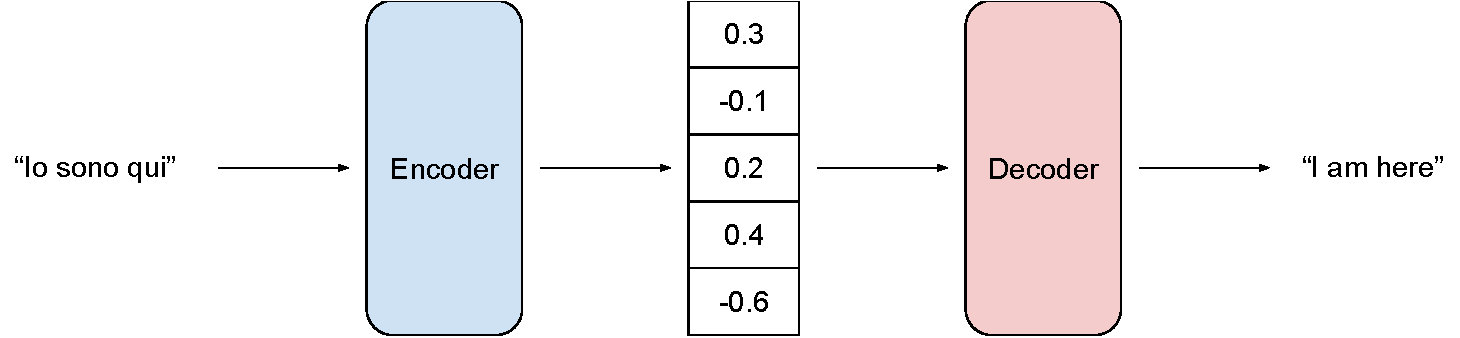
\includegraphics[width=\textwidth]{immagini/stato_arte/encoder_decoder}
\caption{Schema semplificato di un'architettura encoder-decoder che traduce da italiano a inglese}
\label{fig:art_encdec}
\end{figure}

L'idea che gli approcci in questa sezione propongono è quindi quella di trattare il problema della correzione degli errori come un problema di traduzione di sequenze: dato il dominio $E$ delle sequenze contenenti errori, e il dominio $C$ delle sequenze corrette (detto anche Ground Truth, abbreviato GT), il modello seq2seq che effettua la traduzione può essere visto come la seguente funzione:
\begin{equation}
M: E \rightarrow C
\end{equation}
Allo stesso modo, ogni modello necessita prima di essere allenato con corpus parallelo dove ad ogni sequenza $e \in E$ corrisponde un sequenza corretta $c \in C$.

\paragraph{Modelli Word Based e Character based} Come si è visto, i modelli seq2seq trasformano una sequenza in un'altra sequenza. In base al tipo di elementi che compongono tali sequenze, è possibile descrivere due tipologie di modelli:
\begin{itemize}
\item Modelli Word Based (da qui in poi riferiti come WB): in questo tipo modelli un elemento corrisponde ad una parola, o meglio, ad un token. Questo tipo di approcci richiede quindi che tutte le sequenze in $E$ e in $C$ siano tokenizzate. Inoltre, prima dell'allenamento, è necessario estrarre i dizionari della lingua d'origine e della lingua target dai corpora utilizzati.
\item Modelli Character Based (da qui in poi riferiti come CB): in questo tipo di modelli un elemento corrisponde ad un carattere. Prima del training, è necessario estrarre il set di caratteri della lingua d'origine e della lingua target dai corpora utilizzati.
\end{itemize}
Da un'analisi della letteratura, si evince come i modelli CB siano generalmente preferiti per il task dell'OCR Post-Processing\cite{mokhtar2018ocr,hamalainen2019paft,nguyen2020neural,
nastase2018correction,duong2020unsupervised,amrhein2018supervised}.
In \cite{mokhtar2018ocr} viene proposto un confronto sullo stesso corpus fra due architetture molto simili, la prima WB e la seconda CB. Nello studio, gli autori concludono come l'architettura character based produca risultati significativamente migliori. I modelli CB infatti riescono a correggere gli errori a livello di carattere, e ciò comporta i seguenti vantaggi:
\begin{itemize}
\item A differenza dei modelli WB, i modelli CB possono correggere anche errori in parole non presenti nel dizionario estratto.
\item Rispetto ai modelli WB, sono richiesti meno dati durante la fase di allenamento.
\end{itemize}


\paragraph{Approcci basati su NMT}
Il primo approccio presentato è quello descritto in \cite{nguyen2020neural}. Nella soluzione presentata gli autori utilizzano il tool OpenNMT\cite{klein2017opennmt} per allenare un modello CB. Il modello è allenato sia con coppie di sequenze identiche (quindi senza errori) che con sequenze dove la frase acquisita tramite OCR e la GT differiscono. Per queste ultime è adottata la seguente strategia di data augmentation: per ogni errore, si costruiscono cinque 5-gram con il token errato e i suoi token vicini facendo scorrere una finestra sopra la sezione di testo contenente il token errato. In questo modo si producono 5 sequenze diverse che possono essere usate per il training, evitando di un avere un modello con troppo bias verso le sequenze senza errori. L'approccio per la correzione si divide dunque in due fasi: un prima fase di error detection utilizza un modello BERT (si rimanda il lettore alla \autoref{sec:art_bert}) messo a punto per la classificazione per individuare gli errori nelle sequenze; una seconda fase di error correction invece utilizza il modello di NMT allenato precedentemente per correggere gli errori.\\
In \cite{amrhein2018supervised} si utilizza una metodologia simile per il training del modello, sviluppato con il framework Nematus\cite{sennrich2017nematus}. Questo approccio utilizza una tecnica chiamata "factored NMT", utilizzata anche in \cite{nguyen2020neural}, che permette di aggiungere informazioni strutturate alle sequenze in input. Ad esempio, è possibile aggiungere ad ogni carattere della sequenza informazioni sull'identificativo e l'anno del corpus di provenienza. Ciò permette di usare più corpora eterogenei per l'allenamento di un solo modello, aumentando così i dati a disposizione.\\
\cite{nastase2018correction} propone invece un approccio per correggere unicamente i word segmentation errors (si rimanda il lettore alla \autoref{sec:met_introduzione}), ovvero errori introdotti da spazi spuri che influiscono sulla segmentazione del testo. La metodologia proposta allena un modello su coppie di sequenze così composte: la sequenza target è una sequenza corretta senza errori; la sequenza di input invece è la sequenza target senza spaziature. In questo modo, il modello è allenato per inserire correttamente gli spazi e può essere usato per correggere i word segmentation error.\\
In \cite{hamalainen2019paft} si propone invece un approccio per il post processing e l'allenamento di un modello di NMT senza disporre di un corpus parallelo. L'approccio propone di allenare modello Word2Vec direttamente sul corpus contenente gli errori introdotti dal software di OCR. Dopodiché, per ogni parola estratta corretta (la correttezza è verificata attraverso un dizionario) si usa il modello Word2Vec per trovare le parole semanticamente più simili. Di queste, quelle con distanza di Levenshtein minore o uguale di 3 sono considerate versioni errate della parola corretta. Successivamente, le coppie di parole corrette e parole versione errate sono usate per allenare il modello di NMT, che è poi utilizzato per la correzione. Dato che il risultante modello è allenato per la correzione di singole parole, gli errori di segmentazione non vengono corretti. Inoltre, si rende necessaria una fase di error detection basata su un dizionario. \\
L'approccio proposto è ulteriormente sviluppato in \cite{duong2020unsupervised}. Gli autori procedono sempre con la creazione di un corpus parallelo per l'allenamento di un modello di NMT, ma con una diversa strategia. In questo caso si parte da sequenze senza errori, che fungono da input per l'allenamento, e si creano sequenze target mediante l'introduzione di errori in maniera controllata. Inoltre, in questo caso, le sequenze usate per l'allenamento sono degli 5-gram centrati sulla parola errata, con lo scopo di fornire un maggior contesto per migliorare la correzione.


\subsection{Approcci basati su BERT}
\label{sec:art_bert}
%https://towardsdatascience.com/bert-explained-state-of-the-art-language-model-for-nlp-f8b21a9b6270
\paragraph{BERT}
BERT\cite{devlin2018bert} (Bidirectional Encoder Representation from Transformers) è un'architettura per la costruzione di modelli linguistici sviluppata da Google sulla base dei modelli transformers. Una delle differenze fra BERT e un transformer base consiste nella sola presenza di un encoder. Infatti, essendo BERT progettato solo per la modellazione linguistica (e non per la trasformazione di sequenze), non si rende necessaria la presenza di un decoder. Inoltre, a differenza dei modelli direzionali, in cui l'encoder legge il testo in input da sinistra verso desta o viceversa, l'encoder di BERT legge l'intera sequenza all'unisono. Ciò consente al modello di comprendere il contesto di una parola in base al testo a destra e sinistra di quest'ultima. I modelli BERT sono pre-allenati minimizzando la perdita combinata per i task di Masked Language Modelling (MLM) (\autoref{sec:met_BERT_MLM}) e Next Sentence Prediction (NSP). Dopo la fase di pre-allenamento è possibile eseguire il fine-tuning del modello per uno specifico task di NLP, come Classification, Question Answering e Named Entity Recognition (NER).

\paragraph{Approcci basati su BERT}
In \cite{nguyen2020neural}  gli autori eseguono il fine tuning di un modello BERT per eseguire error detection in un dataset in lingua inglese. Ciò avviene dividendo in un primo momento la frase in input in sub-token tramite WordPiece. Il modello BERT classifica quindi i subtoken come validi o non validi: i token che contengono subtoken non validi sono segnalati quindi come errore.\\
In \cite{OCRMaskFilling} gli autori usano una combinazione di BERT e FastText per generare possibili candidati per la correzione di errori introdotti da software OCR in testi in lingua inglese. Limitandosi ai 50 candidati più probabili prodotti con entrambi i metodi, la giusta correzione è presente fra i candidati nel 71\% dei casi. Non è tuttavia proposto un metodo per scegliere il candidato corretto.\\
In \cite{zhang2020spelling} gli autori combinano un neural network di classificazione binaria per l'error detection e un'ulteriore neural network basato su BERT per l'error correction. I token (che in questo caso sono caratteri, dato che l'approccio lavora su testi in lingua cinese)  marcati come errore sono mascherati dal correction network, che propone e sceglie successivamente le soluzioni con più probabilità di essere corrette. I due network sono allenati congiuntamente con un approccio end-to-end, con la loss function che è data da una combinazione lineare delle loss function di correction e detection network.
























\chapter{Dataset e Perturbazione}
\label{sec:dataset}
In questo capitolo è descritto il processo di creazione del dataset usato per valutare il sistema di correzione sviluppato.\\
Nella \autoref{dst:intro} sono discussi gli obiettivi e le caratteristiche che il dataset deve avere. Nella \autoref{dst:creazione} sono delineate la metodologia di creazione e la struttura del dataset. Nella \autoref{dst:perturbazione} è descritto il processo introduzione di errori all'interno delle frasi per simularne l'acquisizione tramite OCR, detto perturbazione. Nella \autoref{dst:configurazione} infine, sono discussi i parametri e la configurazione del dataset.
\section{Introduzione}
\label{dst:intro}
Lo sviluppo di un sistema di OCR post-processing non può prescindere dall'esecuzione di test per valutare, migliorare e confrontare le soluzioni adottate. Ciò rende necessario l'utilizzo di un dataset sul quale poter eseguire tutte le batterie di test necessarie. Tale dataset deve inoltre essere strutturato in modo tale da permettere di calcolare facilmente le metriche descritte nella \autoref{sec:test_metriche}. Se infatti lo scopo di un sistema di OCR post-processing è quello di correggere gli errori introdotti dai software di OCR, è necessario conoscere la posizione degli errori per controllare se siano stati corretti o meno.\\
La soluzione più semplice a questo problema è quella di disporre, per ogni frammento del dataset, sia del testo acquisito tramite OCR (e quindi contenente errori), sia del testo originale, detto anche ground truth. Non è però semplice trovare dataset di questo tipo, specialmente se in lingua italiana. Spesso, infatti, è necessario che la ground truth sia acquisita manualmente con un grosso dispendio di tempo e risorse: a causa di ciò, questo approccio non è stato considerato percorribile ai fini della tesi.\\
Si è invece deciso di adottare un approccio differente, che consiste nell'introduzione artificiale di errori all'interno di testo nativamente digitale (e quindi senza errori) per simularne l'acquisizione tramite OCR. I vantaggi del processo appena descritto, detto "perturbazione", sono riassumibili nei seguenti punti:
\begin{itemize}
 \item Produrre il dataset, una volta definita la funzione che esegue la perturbazione, è molto meno oneroso in termini di tempo e risorse. L'unico requisito è quello di procurarsi una collezione sufficientemente ampia di testo in formato digitale. Ciò è relativamente semplice, e può essere fatto, ad esempio, tramite web scraping. 
 \item \E\ possibile definire arbitrariamente l'intensità e la tipologia degli errori nel testo tramite l'uso di diverse funzioni di perturbazione. Ciò permette, dato un singolo testo di partenza, di ottenere testi con diverse intensità e tipologie di errori. In questo modo si rende possibile valutare le performance del sistema di OCR post-processing al variare delle condizioni del testo dato in input.
\end{itemize}
Il principale rischio che si corre utilizzando l'approccio appena descritto risiede nel fatto che il testo perturbato potrebbe non rispecchiare fedelmente gli errori presenti in testo acquisito realmente tramite software di OCR.

\vfill
\section{Creazione del dataset}
\label{dst:creazione}
Il dataset di partenza è una collezione di 15073 documenti in formato JSON, ottenuti mediante il web scraping del sito ufficiale del vaticano \url{www.vatican.va}. I documenti contengono preghiere, lettere, discorsi, encicliche ecc. editi da figure ecclesiastiche dal 1439 al 2021.\\
Ogni documento è caratterizzato dalla struttura descritta in \autoref{tab:dst_docstrut}.


\begin{table}[H]
\centering
\begin{tabular}{ll}
\textbf{Nome campo} & \textbf{Contenuto} \\ \hline
title & Titolo del documento \\
description & Insieme di keyword del documento\\
author & Autore del testo nel documento \\
creator & Coincide con author \\
language & Codice della lingua del documento (es. it, fr) \\
date & Data di redazione del documento \\
url & Url da cui è stato il documento \\
class & Tipologia di documento (es. discorso, preghiera...)\\
text & Testo completo estratto dal documento (titolo compreso)\\
url\_references & Link al feed RSS del sito del vaticano \\
text\_references & Posizione della pagina nella gerarchia del sito\\
italic & Testo estratto in corsivo nella pagina \\
paragraphs & Testo estratto diviso in paragrafi contenenti id e testo
\end{tabular}
\caption{Struttura di un documento nel dataset}
\label{tab:dst_docstrut}
\end{table}

Dato il dataset descritto, l'obiettivo è quello di trasformalo in un formato consono al testing. Nello specifico, è necessario frammentare il testo contenuto nei documenti in frasi di lunghezza minima e massima predeterminate. Le ragioni di questa decisione sono approfondite nel \autoref{sec:test}, ma, in breve, spezzare il testo in frammenti più piccoli facilita il processo di allineamento delle frasi e quindi la valutazione delle correzioni. Per ognuno dei frammenti si vogliono poi produrre più versioni perturbate con diverse funzioni di perturbazione. Infine, è necessario che le frasi siano accompagnate da dei metadati che consentano la ricomposizione del testo originale mediante il riordinamento dei frammenti.\\
La creazione del dataset per il testing, descritta nelle prossime sezioni, segue dunque le seguenti fasi:
\begin{enumerate}
\item Filtraggio lingue
\item Estrazione
\item Frammentazione
\item Filtraggio paragrafi
\item Perturbazione
\item Riduzione
\end{enumerate}

\paragraph{Filtraggio lingue}
In questa fase vengono filtrati tutti i documenti non presenti fra lingue scelte. Dato l'insieme dei documenti $D$ e l'insieme delle lingue consentite $L$, l'insieme filtrato dei documenti $D_{fl}$ si ottiene come segue:
\begin{equation}
D_{fl} = \{d\ \forall d \in D\ |\ \textit{language}_d \in L  \} 
\end{equation}
dove, dato un documento $d \in D$, $\textit{language}_d$ è la lingua in cui è redatto. Le lingue scelte per la creazione del dataset sono elencate nella \autoref{dst:configurazione}.

\paragraph{Estrazione}
In questa fase sono scartati i campi superflui ai fini del testing, e sono mantenuti solo i paragrafi assieme ad alcuni metadati utili a ricomporre il testo originale in seguito. \E\ possibile formalizzare la prima parte di questa fase come segue:
\begin{equation}
D_{es1} = \{ meta({paragraphs}_d)\ \forall d \in D  \}
\end{equation}
dove la funzione $meta$ aggiunge ai paragrafi in ${paragraphs}_d$ l'id del documento di provenienza. Si ottiene quindi un insieme di insiemi di paragrafi, dove ogni paragrafo è strutturato come in \autoref{tab:dst_parstrut}.

\begin{table}[H]
\centering
\begin{tabular}{ll}
\textbf{Nome campo} & \textbf{Contenuto} \\ \hline
text  & Testo contenuto nel paragrafo\\
parId & Codice del paragrafo all'interno del documento \\
docId & Codice del documento di provenienza del paragrafo.
\end{tabular}
\caption{Struttura di un paragrafo}
\label{tab:dst_parstrut}
\end{table}

La fase di estrazione è completata appiattendo le liste di paragrafi nell'insieme $D_{es1}$ 
\begin{equation}
D_{es} = \bigcup\limits_{p \in D_{es1}} p
\end{equation}
$D_{es}$ contiene quindi tutti i paragrafi del dataset iniziale strutturati come mostrato in \autoref{tab:dst_parstrut}.



\paragraph{Frammentazione}
Lo scopo di questa fase è quello di scomporre i paragrafi estratti nella fase precedente in frammenti più brevi, detti frasi, con le seguenti caratteristiche:
\newcommand{\lmin}{$l_{min}$}
\newcommand{\lmax}{$l_{max}$}
\begin{itemize}
\item Ogni frase è disgiunta dalla altre frasi estratte dal medesimo paragrafo.
\item Ogni frase è compresa fra una lunghezza minima \lmin\ e una lunhezza massima \lmax\ (\autoref{dst:configurazione}).
\end{itemize}

Dato quindi il testo di un paragrafo $text_p$, la frammentazione avviene secondo la seguente procedura:

\begin{enumerate}
\item Se la lunghezza di $text_p$ è minore di \lmin, non si procede e si scarta la stringa.
\item Si divide $text_p$ su un segno di punteggiatura fra i seguenti: "?", "!", ";", ":", ".", ",". Se sono disponibili più opzioni (ovvero più punti in cui è possibile dividere su segni di punteggiatura) si divide nel punto minore o uguale a \lmax\ che più si avvicina al valore di \lmax. La parte a sinistra del punto di divisione è una frase estratta. La parte a destra invece viene riutilizza come input della procedura di frammentazione, tornando al punto 1. Se non fosse possibile eseguire alcuna divisione, si passa al punto successivo.
\item Si divide $text_p$ su uno spazio. Se sono disponibili più opzioni (ovvero più punti in cui è possibile dividere su uno spazio) si divide nel punto minore o uguale a \lmax\ che più si avvicina al valore di \lmax. La parte a sinistra del punto di divisione è una frase estratta. La parte a destra invece viene riutilizza come input della procedura di frammentazione, tornando al punto 1. Se non fosse possibile eseguire alcuna divisione, si passa al punto successivo.
\item Se la lunghezza di $text_p$ è minore di \lmax, $text_p$ è aggiunto alle frasi estratte. Altrimenti, si divide $text_p$ in posizione \lmax. La parte a sinistra del punto di divisione è una frase estratta. La parte a destra invece viene riutilizza come input della procedura di frammentazione, tornando al punto 1. 
\end{enumerate}

La procedura appena descritta fa in modo che i frammenti approssimino il più possibile \lmax, evitando il più possibile introdurre errori. Spezzare un paragrafo nel mezzo di una parola, ad esempio, andrebbe a creare due frammenti contenenti degli errori (uno sulla parola finale del primo, l'altro sulla parola iniziale del secondo.\\
Durante la frammentazione ogni frammento ritiene i metadati relativi al documento e al paragrafo di appartenenza. In più, si aggiunge un ulteriore campo per tenere traccia della posizione del frammento all'interno del paragrafo di appartenenza. In questo modo, è possibile ricomporre un documento in secondo momento. Ogni frase prodotta rispetta il seguente schema:
\begin{table}[H]
\centering
\begin{tabular}{ll}
\textbf{Nome campo} & \textbf{Contenuto} \\ \hline
text  & Testo contenuto nella frase\\
parId & Codice del paragrafo di provenienza \\
docId & Codice del documento di provenienza.\\
parPos & Posizione della frase all'interno del paragrafo di provenienza\\
\end{tabular}
\caption{Struttura di una frase}
\label{tab:dst_frasestrut}
\end{table}

La frase di frammentazione si può quindi formalizzare in due step. Nel primo step, ogni paragrafo viene frammentato nella lista delle sue frasi:
\begin{equation}
D_{fr1} = \{ extr(p)\ \forall p \in D_{es}  \}
\end{equation}
dove $extr$ è la funzione che estrae le frasi secondo la procedura descritta precedentemente, producendo un insieme di frasi strutturate come mostrato in \autoref{tab:dst_frasestrut}. Nel secondo step si appiattisce l'insieme di insiemi che si è andato a creare, per ottenere insieme di frasi:
\begin{equation}
D_{fr} = \bigcup\limits_{f \in D_{fr1}} f
\end{equation}

\paragraph{Filtraggio paragrafi}
Lo scopo di questa fase è quello di rimuovere dal dataset tutti le frasi che appartengono al primo o all'ultimo paragrafo di un documento. Ciò si rende necessario perchè questi paragrafi spesso contengono intestazioni o piè di pagina ripetitivi andrebbero a sporcare il dataset. Ad esempio, l'ultimo paragrafo contiene spesso una frase simile  a \textit{"© Copyright 2004 - Libreria Editrice Vaticana"}, mentre il primo spesso contiene solamente una data.\\
\E\ definita la seguente funzione $\textit{maxPar}$ che, data una frase $f \in D_{fr}$, indica se $f$ appartiene all'ultimo paragrafo del documento da cui è stata estratta:
\begin{equation}
  maxPar(f) =
    \begin{cases}
      1 & \text{se $f$ appartiene all'ultimo paragrafo di $docId_f$}\\
      0 & \text{altrimenti}
    \end{cases}       
\end{equation}
L'operazione di filtraggio dei paragrafi può quindi essere formalizzata come segue:
\begin{equation}
D_{fp} = \{ f \ \forall f \in D_{fr}\ |\  parId_{f} \neq 0 \wedge maxPar(f) = 0     \}
\end{equation}

\paragraph{Perturbazione}
Durante la fase di perturbazione, per ogni frase del dataset sono generate le sue versioni perturbate. Ogni versione perturbata di una frase viene generata da una diversa funzione di perturbazione applicata alla frase stessa. Il funzionamento delle funzioni di perturbazione è spiegato nella \autoref{dst:perturbazione}, mentre le esatte funzioni per la creazione del dataset sono elencate nella \autoref{dst:configurazione}.\\
Viene chiamata $F_p$ la lista $[p_1,...,p_n]$ delle funzioni di perturbazione utilizzate, in cui ogni $p_i$ è identificata da un codice. Data una stringa di testo $s$, la sua versione perturbata dalla funzione $p_i$ corrisponde a $p_i(s)$.\\
Data quindi una frase $f \in D_{fr}$ strutturata come in \autoref{tab:dst_frasestrut}, e lista delle funzioni di perturbazione $F_p$, si definisce come $P_{list}$ l'insieme delle frasi perturbate $[p_1(text_f),...,p_n(text_f)]$ la cui rappresentazione è schematizzata in \autoref{tab:dst_frasepert}.

\begin{table}[H]
\centering
\begin{tabular}{ll}
\textbf{Codice funzione perturbazione} & \textbf{Frase perturbata} \\ \hline
$nome\_func_1$ & $ p_1(f)$\\
$nome\_func_2$ & $ p_2(f)$\\
... &  ...\\
$nome\_func_n$ & $ p_n(f)$\\
\end{tabular}
\caption{Struttura delle frasi perturbate}
\label{tab:dst_frasepert}
\end{table}

Si definisce inoltre la funzione $applyPert$ che, data una frase $f \in D_{fr}$, produce un sample aggiungendo a $f$ un campo con le sue versioni perturbate della frase originale. Un sample è strutturato come in \autoref{tab:dst_samplestrut}.

\begin{table}[H]
\centering
\begin{tabular}{ll}
\textbf{Nome campo} & \textbf{Contenuto} \\ \hline
text  & Testo contenuto nella frase non perturbata\\
parId & Codice del paragrafo di provenienza \\
docId & Codice del documento di provenienza.\\
parPos & Posizione della frase all'interno del paragrafo di provenienza\\
perturbed & Frasi perturbate ($[p_1(text_f),...,p_n(text_f)]$)
\end{tabular}
\caption{Struttura di una frase}
\label{tab:dst_samplestrut}
\end{table}


La fase di perturbazione può quindi essere formalizzata come segue:
\begin{equation}
D_{pe} = \{applyPert(f)\ \forall f \in D_{fp}\}
\end{equation}

\paragraph{Riduzione}
Lo scopo della fase di riduzione è quello di creare una versione ridotta del dataset, ovvero di ridurne il numero di elementi. Ciò è reso necessario dal fatto che il testing può essere significativamente oneroso in termini di tempo e risorse, specialmente su dataset troppo ampi.\\
Data quindi la dimensione del dataset ridotto $n$ (i cui valori sono specificati nella \autoref{dst:configurazione}), il dataset $D_{re}$ è un sottoinsieme di $n$ elementi estratti casualmente da $D_{pe}$:
\begin{equation}
D_{re} \subset D_{pe} \wedge |D_{re}| = n
\end{equation}
Dopo aver eseguito la fase di riduzione, la costruzione del dataset può dirsi completata.


\section{Perturbazione}
\label{dst:perturbazione}
Data una stringa $s$, lo scopo del processo di perturbazione è quello produrre una stringa $s\prime$ nella quale sono introdotti degli errori per simulare l'acquisizione del testo tramite OCR. Per permettere l'introduzione controllata e a diverse intensità degli errori è stato sviluppato un sistema modulare e componibile, che sarà illustrato in questa sezione.

\subsection{Moduli di perturbazione}
\label{dst:modpert}
La componente base del sistema di perturbazione è il modulo di perturbazione. Un modulo di perturbazione non è altro che una funzione che modella l'inserimento di una specifica tipologia di errore. Ciò significa che per ogni tipologia di errore modellata si rende necessaria la creazione di un modulo di perturbazione. Ad esempio, è possibile definire un modulo di perturbazione che modelli la sostituzione di alcuni caratteri, o un modulo che inserisca della punteggiatura spuria. \\
Tutti i moduli di perturbazione, data una lista ordinata di token, introducono errori mediante la modifica, la divisione, l'unione o la cancellazione di uno o più token. \\
Data una lista di token $list_t = [t_1,...,t_n]$,
Il funzionamento di un modulo di perturbazione si può dividere nelle seguenti tre fasi:

\begin{enumerate}
	\item \textbf{Raggruppamento}: I token sono raggruppati in gruppi consecutivi e disgiunti di $k$ elementi, dove $k$ varia a seconda della tipologia di modulo di perturbazione. \\
La fase di raggruppamento è quindi definita come segue:
\begin{equation}
group: [t_1,...,t_n] \rightarrow [g_1,...,g_q]
\end{equation}
dove ogni $g_i$ è un gruppo di token $[t_1,..., t_k  ]$ e $q = \lceil n/k \rceil$.\\
	
Ad esempio, data la lista di token \textit{['Nel', 'mezzo', 'del', 'cammin', 'di', 'nostra', 'vita']} e $k = 2$, i token sono raggruppati nel seguente modo: \textit{['Nel', 'mezzo'], ['del', 'cammin'], ['di', 'nostra'], ['vita']}.
	
	\item \textbf{Perturbazione}: Ogni tipologia di modulo di perturbazione è caratterizzata da una specifica funzione di perturbazione $f_{pert}$
\begin{equation}
f_{pert}: [t_1,..., t_k  ] \rightarrow [t'_1,..., t'_j]
\end{equation}
che introduce errori mediante la modifica, la divisione, l'unione o la cancellazione dei token in un determinato gruppo, con una probabilità $p$ definita per ogni modulo. Un qualsiasi gruppo di token $g \in [g_1,...,g_q]$ viene perturbato o meno secondo la seguente funzione:
\begin{equation}
f_{map}(g) =
    \begin{cases}
      f_{pert}(g) & \text{con probabilità $p$}\\
      g & \text{con probabilità $1-p$}
    \end{cases}  
\end{equation}
\E\ quindi possibile definire la fase di perturbazione come:
\begin{equation}
pert: [g_1,...,g_q] \rightarrow [g\prime_1,...,g\prime_q]
\end{equation}
dove $g\prime_i = f_{map}(g_i)\ \forall i \in [1..q]$.


Ad esempio, si supponga di avere un modulo in cui $f_{pert}$ sia definita come:
\begin{equation}
f_{ex}([t_1,t_2]) = [t_1 \frown t_2]
\end{equation}
La funzione appena definita concatena i due token all'interno di gruppo, restituendo un gruppo formato da un solo token. Si consideri l'esempio nel punto precedente, e si supponga che l'unico gruppo affetto da perturbazione sia il secondo. Si ha quindi che $f_{pert}(\textit{['del', 'cammin']}) = \textit{['delcammin']}$, e quindi alla fine di questa fase si ottiene: \textit{['Nel', 'mezzo'], ['delcammin'], ['di', 'nostra'], ['vita']}.

\item \textbf{Appiattimento}: la fase di appiattimento è l'opposto di quanto avviene durante il raggruppamento. I gruppi di token sono raggruppati nuovamente in un'unica lista:
\begin{equation}
flat: [g\prime1,...,g\prime_q] \rightarrow [t_1,...,t_m]
\end{equation}
dove $m$ potrebbe coincidere o meno con $n$ a seconda del tipo di perturbazione avvenuta.\\
Riprendendo l'esempio precedente, il risultato di questa fase è: \textit{['Nel', 'mezzo', 'delcammin', 'di', 'nostra', 'vita']}
\end{enumerate}

Come si può notare, un modulo riceve in input una lista di token e fornisce in output un'altra lista di token. Ciò rende possibile concatenare più moduli, per introdurre più di un tipo di errore all'interno di una sequenza di token. Questa eventualità è descritta nella \autoref{sec:dst:pipeline} e nella \autoref{sec:dst:superpipeline}.\\
Quanto descritto finora non basta a soddisfare lo scopo della perturbazione, che è quello di trasformare una stringa in una nuova stringa contenente degli errori. Tale funzione è resa possibile dai moduli speciali, che sono approfonditi nella \autoref{sec:dst_modspec}.\\
Dal funzionamento dei moduli di perturbazione si evince come la funzione $f_{pert}$ caratterizzi il modulo modellando il tipo di errore che esso va ad introdurre. Sono quindi stati creati i seguenti moduli, ognuno dei quali è caratterizzato da una diversa funzione di perturbazione:

\newcommand{\mss}{$M_{ss}$}
\newcommand{\mps}{$M_{ps}$}
\newcommand{\mpi}{$M_{pi}$}
\newcommand{\mhm}{$M_{hm}$}
\newcommand{\mcr}{$M_{cr}$}

\begin{itemize}
\item Modulo di space splitting (\mss)
\item Modulo di punctuation splitting (\mps)
\item Modulo di punctuation insertion (\mpi)
\item Modulo di hyphen merging (\mhm)
\item Modulo di characters replacement (\mcr)
\end{itemize}

Ognuno di questi moduli è stato creato per modellare un particolare tipo di errore. Le tipologie di errore modellate sono state decise in base all'analisi di documenti il cui testo è stato acquisito tramite OCR. Più nello specifico, si tratta delle trascrizioni dei dibattiti parlamentari della prima e della seconda legislatura della repubblica italiana.

\subsubsection{Modulo di space splitting}
Il modulo di space splitting modella l'errore in cui le lettere di una parola sono intramezzate da degli spazi. Siccome la perturbazione avviene su un singolo token, i token in input sono raggruppati in gruppi di un token ($k = 1$). Si definisce dunque la funzione di perturbazione del modulo:
\begin{equation}
f_{pert\_split}([t_1]) = [f_{split}(t_1)]
\end{equation}
in cui $f_{split}$ è la funzione che aggiunge uno spazio dopo ogni carattere di un token.
\paragraph{Esempi}
\begin{equation}
f_{pert\_split}(["cammin"]) = ["c\ a\ m\ m\ i\ n\ "]
\end{equation}
\begin{equation}
f_{pert\_split}(["nostra"]) = ["n\ o\ s\ t\ r\ a\ "]
\end{equation}

\subsubsection{Modulo di punctuation splitting}
Il modulo di punctuation splitting modella l'errore in cui una o più occorrenze di un segno di punteggiatura intramezzano i caratteri di una parola.
Siccome la perturbazione avviene su un singolo token, i token in input sono raggruppati in gruppi di un token ($k = 1$). Si definisce dunque la funzione di perturbazione del modulo:
\begin{equation}
f_{pert\_punctsplit}([t_1]) = [f_{punctsplit}(t_1,punct)]
\end{equation}
Assumendo che:
\begin{itemize}
\item $punct$ sia il segno di punteggiatura che è intramezzato agli spazi,
\item un token $t$ sia una sequenza di caratteri $[c_1,...,c_n]$, ovvero $|t| = n$,
\item sia definito un numero casuale $x \in \mathbb{N}\ |\ 1 \leq x \leq n$
\end{itemize}
è possibile definire $f_{punctsplit}$ come:
\begin{equation}
f_{punctsplit}(t,punct) = 
\begin{cases}
	[c1,...,c_x] \frown\ punct \frown f_{punctsplit}([c_{x+1},...,c_n],punct)&\text{se $x < |t|$}\\
	t	&\text{se $x \geqslant |t|$}
\end{cases}
\end{equation}
Informalmente, la funzione aggiunge un carattere $punct$ ogni $x$ caratteri all'interno di $t$.

\paragraph{Esempi}
\begin{equation}
f_{punctsplit}(\textit{"cammin"},\textit{","}) = \textit{"ca,mm,in"}\ (x = 2)
\end{equation}
\begin{equation}
f_{punctsplit}(\textit{"mezzo"},\textit{","}) = \textit{"m,e,z,z,o"}\ (x = 1)
\end{equation}


\subsubsection{Modulo di punctuation insertion}
Il modulo di punctuation insertion modella l'errore in cui un segno di punteggiatura è aggiunto fra due token, senza quindi dividere in due un singolo token.
Siccome la perturbazione avviene su un singolo token, i token in input sono raggruppati in gruppi di un token ($k = 1$). Si definisce dunque la funzione di perturbazione del modulo:
\begin{equation}
f_{pert\_insertion}([t_1]) = [t_1, punct]
\end{equation}
dove $punct$ è il segno di punteggiatura da aggiungere.
\paragraph{Esempi} Data la sequenza di gruppi di token \textit{\underline{['Nel']}, ['mezzo'], ['del'], \underline{['cammin']}, ['di'], ['nostra'], ['vita']}, dove i gruppi sottolineati sono quelli da perturbare, e dato $punct = "."$, si ha che:
\begin{equation}
f_{pert\_insertion}(\textit{["Nel"]},\textit{"."}) = \textit{["Nel","."]}\ 
\end{equation}
\begin{equation}
f_{pert\_insertion}(\textit{["cammin"]},\textit{"."}) = \textit{["cammin","."]}\ 
\end{equation}
Quindi, applicata la fase di appiattimento, la sequenza finale risulta: \textit{['Nel'], ['.'], ['mezzo'], ['del'], ['cammin'], ['.'], ['di'], ['nostra'], ['vita']}.

\subsubsection{Modulo di hyphen merging}
Il modulo di hypen merging modella l'errore in cui due parole consecutive vengono unite da un trattino. Dovendo unire due token tra di loro, la perturbazione avviene in gruppi di due token, quindi si ha $k = 2$. Si definisce dunque la funzione di perturbazione del modulo:
\begin{equation}
f_{hyphen}([t_1,t_2]) = [t_1\frown \textit{"-"} \frown t_2]
\end{equation}

\paragraph{Esempio} Data la sequenza di gruppi di 2 token \textit{['Nel', 'mezzo'], ['del', 'cammin'], \underline{['di', 'nostra']}, ['vita']}, dove il gruppo sottolineati sono quello da perturbare, si ha che:
\begin{equation}
f_{hyphen}(\textit{["di", "nostra"]}) = \textit{["di-nostra"]}
\end{equation}
Quindi, applicata la fase di appiattimento, la sequenza finale risulta: \textit{['Nel', 'mezzo'], ['del', 'cammin'], {['di-nostra']}, ['vita']}.

\subsubsection{Modulo di characters replacement}
Il modulo di characters replacement modella l'errore in un cui avviene la cancellazione, l'aggiunta o la sostituzione di uno o più caratteri all'interno di un token. Siccome la perturbazione avviene su un singolo token, i token in input sono raggruppati in gruppi di un token ($k = 1$). Si definisce dunque la funzione di perturbazione del modulo:
\begin{equation}
f_{charrepl}([t_1]) = [f_{alternative}(t_1)]
\end{equation}
Per ogni token $t$ che viene perturbato, esiste un insieme di 5 versioni errate di $t$, detto $A_t = [a_{t1},...,a_{t5}]$, generato sulla base di una distribuzione di errori preesistente. La funzione $f_{alternative}$ rimpiazza $t$ con una delle alternative in $A_t$:
\begin{equation}
f_{alternative}(t) = a_{ti}
\end{equation}
dove $a_{ti} \in A_t$ e $i$ è un numero intero casuale fra 1 e 5.

\paragraph{Esempio} Sia dato il token \textit{"cammin"} e si supponga l'insieme delle versioni errate del token essere $A_{cammin} = [\textit{'cmmin', 'camniin', 'cdmmn', 'camin', 'cammiii'}]$. Si sceglie quindi in modo casuale un token dall'insieme $A_{cammin}$:
\begin{equation}
f_{alternative}(\textit{"cammin"}) = a_{cammin\_2} ="camniin"
\end{equation}


\subsection{Moduli speciali}
\label{sec:dst_modspec}
Come si è visto nella sottosezione precedente, i moduli di perturbazione lavorano su sequenze di token, nelle quali introducono degli errori. \E\ però necessario, come accennato all'inizio della \autoref{dst:perturbazione}, che la perturbazione prenda in input e restituisca come output delle stringhe. Sono quindi definiti due moduli, detti moduli speciali, che hanno lo scopo di convertire una stringa in una sequenza di token e viceversa:
\newcommand{\mto}{$M_{to}$}
\newcommand{\mde}{$M_{de}$}
\begin{itemize}
\item Modulo di tokenizzazione (\mto)
\item Modulo di detokenizzazione (\mde)
\end{itemize}

\subsubsection{Modulo di tokenizzazione}
Il modulo di tokenizzazione ha lo scopo di tokenizzare una qualsiasi stringa $s \in S$ in una lista $[t_1,...,t_n]$ di token:
\begin{equation}
tok: S \rightarrow [t_1,...,t_n]
\end{equation}
\paragraph{Esempio}
Data la frase $s_{ex} = \textit{"Nel mezzo del cammin di nostra vita"}$  
\begin{equation}
tok(s_{ex}) = \textit{['Nel', 'mezzo', 'del', 'cammin', 'di', 'nostra', 'vita']}
\end{equation}

\subsubsection{Modulo di detokenizzazione}
Il modulo di tokenizzazione ha lo scopo di detokenizzare, ovvero di eseguire il processo contrario alla tokenizzazione, una lista di token $[t_1,...,t_n]$ in una stringa $s \in S$.
\begin{equation}
detok: [t_1,...,t_n] \rightarrow S
\end{equation}
\paragraph{Esempio}
Data la sequenza di token $T_{ex} =$ \textit{['Nel', 'mezzo', 'del', 'cammin', 'di', 'nostra', 'vita']}.
\begin{equation}
detok(T_{ex}) = \textit{"Nel mezzo del cammin di nostra vita"}
\end{equation}



\subsection{Pipeline}
\label{sec:dst:pipeline}
Come accennato nelle sottosezioni precedenti, ogni modulo di perturbazione modella un diverso tipo di errore. In realtà, in un testo estratto tramite OCR sono presenti più tipologie di errori. \E\ quindi necessario utilizzare più moduli di perturbazione in sequenza per ottenere una perturbazione verosimile. Considerando che ogni modulo di perturbazione è considerabile come una funzione con dominio e codominio coincidenti $T$ (ogni elemento del dominio e codominio $T$ è una lista di token $[t_1,...,t_n]$ con $ n \in \mathbb{N} \wedge n \geqslant 0$), è possibile concatenare più moduli insieme tramite composizione:
\begin{equation}
m_k \circ m_{k-1} \circ m_{k-2} \circ ... \circ m_1
\end{equation}
dove ogni $m_i$ è istanza di un modulo di perturbazione. La funzione composta non può però trattare stringe, ma solo sequenze di token. Ciò è ovviabile attraverso l'aggiunta dei moduli speciali di tokenizzazione e detokenizzazione all'inizio e alla fine della composizione. La funzione risultante prende il nome di pipeline:
\begin{equation}
Pipeline: detok \circ m_k \circ m_{k-1} \circ m_{k-2} \circ ... \circ m_1 \circ tok
\end{equation}
Data quindi una stringa $s \in S$, la stringa perturbata $s\prime \in S$ è ottenuta come:
\begin{equation}
Pipeline(s) = s\prime
\end{equation}

\paragraph{Esempio}
Si definisca una pipeline $p_{ex}$ composta come indicato in \autoref{tab:dst_pex}.

\begin{table}[H]
\centering
\begin{tabular}{ccccc}
\textbf{Posizione} & \textbf{Nome istanza} & \textbf{Tipo Modulo} & \textbf{p} & \textbf{punct}\\ \hline
1	& $m_{to}$	& \mto	& n.d 	& n.d 	\\
2	& $m_{cr}$	& \mcr	& 0.3	& n.d 	\\
3	& $m_{ss}$	& \mss	& 0.1	& n.d 	\\
4	& $m_{pi}$	& \mpi	& 0.1	& , 	\\
5	& $m_{de}$	& \mde	& n.d 	& n.d 	\\
\end{tabular}
\caption{Struttura della pipeline $p_{ex}$}
\label{tab:dst_pex}
\end{table}

$p_{ex}$ corrisponde dunque alla seguente funzione, schematizzata anche in \autoref{fig:dst_pex}.
\begin{equation}
p_{ex} = m_{de} \circ m_{pi} \circ m_{ss} \circ m_{cr} \circ m_{to}
\end{equation}

\begin{figure}[H]
\centering
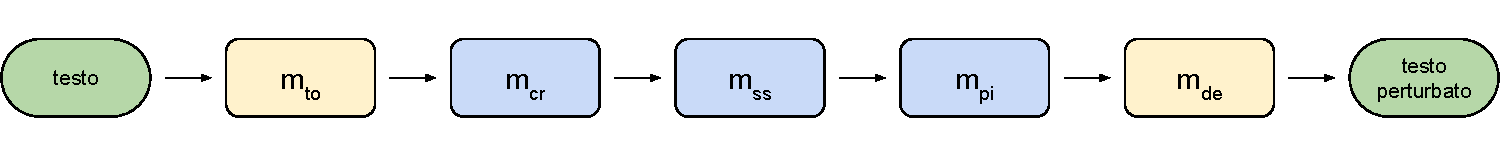
\includegraphics[width=\textwidth]{immagini/dataset/pex}
\caption{Schema della pipeline $p_{ex}$}
\label{fig:dst_pex}
\end{figure}

Data una stringa di esempio $s_{ex} = $ \textit{"Nel mezzo del cammin di nostra vita"}, è mostrata in seguito la sequenza dei passaggi che portano alla perturbazione della frase:
\begin{enumerate}
\setcounter{enumi}{-1}
\item ($s_{ex}$)\\
\textit{"Nel mezzo del cammin di nostra vita"}

\item $m_{to}(s_{ex})$\\
\textit{['Nel', 'mezzo', 'del', 'cammin', 'di', 'nostra', 'vita']}

\item $m_{cr}(m_{to}(s_{ex}))$\\
\textit{['Nel', \underline{'inezzo'}, 'del', \underline{'camniin'}, 'di', 'nostra', 'vita']}

\item $m_{ss}(m_{cr}(m_{to}(s_{ex})))$\\
\textit{['Nel', 'inezzo', 'del', \underline{'c a m n i i n'}, 'di', 'nostra', 'vita']}

\item $m_{pi}(m_{ss}(m_{cr}(m_{to}(s_{ex}))))$\\
\textit{['Nel', 'inezzo', 'del', 'c a m n i i n', 'di', \underline{','} , 'nostra', 'vita']}

\item $m_{de}(m_{pi}(m_{ss}(m_{cr}(m_{to}(s_{ex})))))$\\
\textit{"Nel inezzo del c a m n i i n di, nostra vita"}
\end{enumerate} 

Si sottolinea come questa sia solo una delle possibili perturbazioni di $s_{ex}$: essendoci nella perturbazione una componente aleatoria, ogni esecuzione di una pipeline su uno stesso input può dare risultati diversi.


\subsection{Superpipeline}
\label{sec:dst:superpipeline}
Una pipeline di perturbazione perturba il testo in modo uniforme: ogni frase perturbata con una pipeline $p$ ha una concentrazione di errori simile. Nell'osservazione di testi acquisiti tramite OCR si nota però come la distribuzione degli errori non sia uniforme: si possono incontrare sezioni prive di errori, ma anche parti di testo in cui è presente molto rumore. Ciò è spesso dovuto alle condizioni del documento originale, che in alcune parti può essere più degradato che in altre. Questo comporta che una sola pipeline non può simulare fedelmente gli errori OCR: è necessario variare l'intensità e la modalità di perturbazione per ottenere un risultato più verosimile.\\
Si introduce quindi il concetto di superpipeline. Date:
\begin{itemize}
\item Una lista $\textit{Ppl} = [p_1,...,p_n]$ dove ogni $p_i$ è una pipeline,
\item Una lista di pesi $W = [w_1,...,w_n]$ dove $w_i \in \mathbb{N}$ è il peso associato ad $p_i$,
\end{itemize}
è possibile definire una superpipeline come una funzione che, data una stringa $s \in S$, ne produce una versione perturbata tramite una pipeline $p_{rand}$ scelta casualmente da $\textit{Ppl}$. La probabilità che una pipeline $p_i$ venga scelta corrisponde a:
\begin{equation}
P(p_{rand} = p_i) = \frac{w_i}
{{\sum_{j=0}^{n}}w_j}
\end{equation}


\paragraph{Esempio}
Si definiscono le tre pipeline $p_{ex1},\ p_{ex1},\ p_{ex1}$, rispettivamente in \autoref{tab:dst_pex1}, \autoref{tab:dst_pex2}, \autoref{tab:dst_pex3}. 
\begin{table}[H]
\centering
\begin{tabular}{ccccc}
\textbf{Posizione} & \textbf{Nome istanza} & \textbf{Tipo Modulo} & \textbf{p} & \textbf{punct}\\ \hline
1	& $m_{to}$	& \mto	& n.d 	& n.d 	\\
2	& $m_{cr}$	& \mcr	& 0.5	& n.d 	\\
3	& $m_{de}$	& \mde	& n.d 	& n.d 	\\
\end{tabular}
\caption{Definizione di $p_{ex1}$}
\label{tab:dst_pex1}
\end{table}

\begin{table}[H]
\centering
\begin{tabular}{ccccc}
\textbf{Posizione} & \textbf{Nome istanza} & \textbf{Tipo Modulo} & \textbf{p} & \textbf{punct}\\ \hline
1	& $m_{to}$	& \mto	& n.d 	& n.d 	\\
2	& $m_{cr}$	& \mcr	& 0.3	& n.d 	\\
3	& $m_{hm}$	& \mhm	& 0.1	& n.d 	\\
4	& $m_{de}$	& \mde	& n.d 	& n.d 	\\
\end{tabular}
\caption{Definizione di $p_{ex2}$}
\label{tab:dst_pex2}
\end{table}

\begin{table}[H]
\centering
\begin{tabular}{ccccc}
\textbf{Posizione} & \textbf{Nome istanza} & \textbf{Tipo Modulo} & \textbf{p} & \textbf{punct}\\ \hline
1	& $m_{to}$	& \mto	& n.d 	& n.d 	\\
2	& $m_{cr}$	& \mcr	& 0.3	& n.d 	\\
3	& $m_{ss}$	& \mss	& 0.1	& n.d 	\\
4	& $m_{pi}$	& \mpi	& 0.1	& , 	\\
5	& $m_{de}$	& \mde	& n.d 	& n.d 	\\
\end{tabular}
\caption{Definizione di $p_{ex3}$}
\label{tab:dst_pex3}
\end{table}

Si definisce inoltre la lista dei pesi $W =[1,3,2]$. Quindi, calcolata la somma dei pesi $w_1  + w_2 + w_3 = 6$, si ha che:
\begin{itemize}
\item $p_{ex1}$ è usata con probabilità $w_1 / 6 = 1 / 6 = 0.17$
\item $p_{ex2}$ è usata con probabilità $w_2 / 6 = 3 / 6 = 0.50$
\item $p_{ex3}$ è usata con probabilità $w_3 / 6 = 2 / 6 = 0.33$
\end{itemize}

La superpipeline composta è quindi schematizzabile come mostrato in \autoref{fig:dst_supex}.

\begin{figure}[H]
\centering
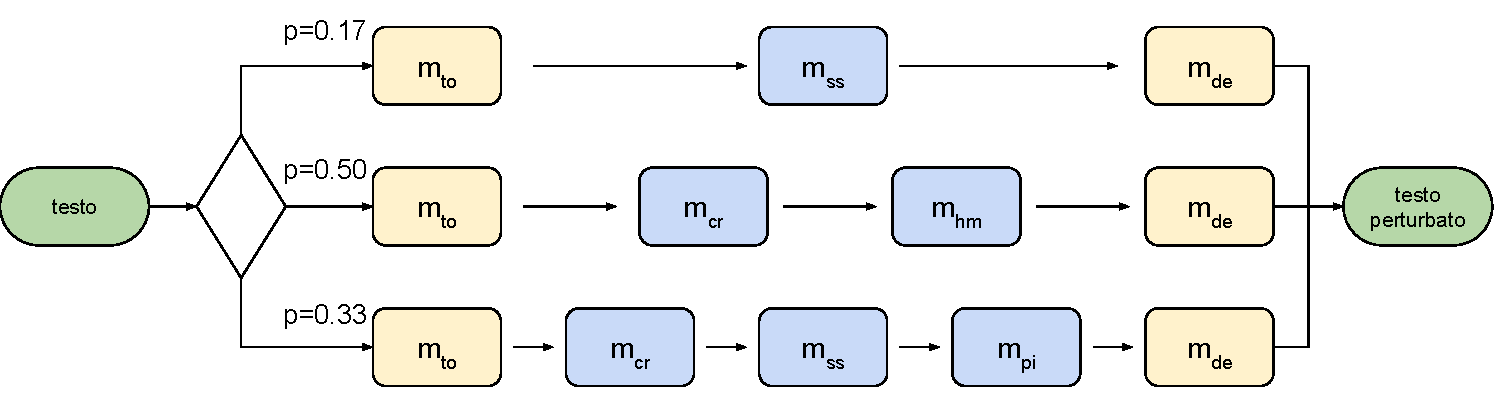
\includegraphics[width=\textwidth]{immagini/dataset/supex}
\caption{Schema della superpipeline descritta nell'esempio}
\label{fig:dst_supex}
\end{figure}



\section{Configurazione}
\label{dst:configurazione}
Nelle precedenti sezioni sono stati descritti la metodologia di creazione del dataset e il funzionamento del sistema di perturbazione. In questa sezione sono invece descritti i parametri usati per il sistema di perturbazione e quindi per la creazione del dataset.

\subsection{Pipeline e Superpipeline}
\label{sec:dst_pipsup}
In questa sottosezione sono definite le superpipeline usate per la perturbazione del dataset e le pipeline che le compongono. Sono state stabilite 3 tipologie di superpipeline, ognuna delle quali ha 3 livelli di intensità:

\begin{itemize}
\item \textbf{Token superpipeline}: sono superpipeline che introducono solo dei word error (\autoref{sec:met_introduzione}), ovvero errori contenuti all'interno di un singolo token che non impattano la tokenizzazione. Le token superpipeline sono identificate dai codici T1, T2, T3, dove T1 e T3 sono rispettivamente la superpipeline che introduce meno errori e quella che ne introduce di più.

\item \textbf{Segmentation superpipeline}: sono superpipeline che introducono solo dei word segmentation error (\autoref{sec:met_introduzione}), ovvero che dividono o uniscono uno o più token e che impattano quindi la tokenizzazione. Le segmentation superpipeline sono identificate dai codici S1, S2, S3, dove S1 e S3 sono rispettivamente la superpipeline che introduce meno errori e quella che ne introduce di più.

\item \textbf{Mixed Pipeline}: sono superpipeline che introducono sia word error che word segmentation error. Le segmentation superpipeline sono identificate dai codici M1, M2, M3, dove M1 e M3 sono rispettivamente la superpipeline che introduce meno errori e quella che ne introduce di più.
\end{itemize}

In tutto quindi sono definite 9 superpipeline (T1, T2, T3, S1, S2, S3, M1, M2, M3): questo numero permette di avere una buona granularità tenendo comunque contenuti i tempi durante la fase di testing.

\subsubsection{Pipeline}
Le superpipeline appena descritte sono formate dalla combinazione di più pipeline. Sono definiti tre tipi di pipeline:
\begin{itemize}
\item Token pipeline
\item Segmentation pipeline
\item Mixed pipeline
\end{itemize}
ognuna di queste tipologie di pipeline introduce gli stessi tipi di errore delle omonime superpipeline. Per ogni tipologia di pipeline sono definite 3 pipeline, ognuna della quali ha li stessi moduli con probabilità diverse.

\paragraph{Token pipeline} Una token pipeline è formata dai moduli presenti nella seguente \autoref{tab:dst_tkpip}:

\begin{table}[H]
\centering
\begin{tabular}{cccc}
\textbf{Posizione} & \textbf{Tipo Modulo} & \textbf{punct}\\ \hline
1	& \mto	& n.d 	\\
2	& \mcr	& n.d 	\\
3	& \mde	& n.d 	\\
\end{tabular}
\caption{Moduli presenti in una token pipeline}
\label{tab:dst_tkpip}
\end{table}

In \autoref{tab:dst_tkpipdef} sono definite le tre token pipeline. Nella tabella, $p_i$ indica la probabilità associata al modulo in posizione $i$.

\begin{table}[H]
\centering
\begin{tabular}{cccc}
\textbf{Codice} & \boldmath{$p_1$} & \boldmath{$p_2$} & \boldmath{$p_3$}  \\ \hline
$tok_1$	& n.d	& 0.1	& n.d 	\\
$tok_2$	& n.d	& 0.3	& n.d 	\\
$tok_3$	& n.d	& 0.3	& n.d 	\\
\end{tabular}
\caption{Definizione delle tre token pipeline}
\label{tab:dst_tkpipdef}
\end{table}



\paragraph{Segmentation pipeline}
Una segmentation pipeline è formata dai moduli presenti nella seguente \autoref{tab:dst_sgpip}:

\begin{table}[H]
\centering
\begin{tabular}{cccc}
\textbf{Posizione} & \textbf{Tipo Modulo} & \textbf{punct}\\ \hline
1	& \mto	& n.d 	\\

2	& \mhm	& n.d 	\\
3	& \mps	& , (virgola)	\\
4	& \mss	& n.d 	\\
5	& \mpi	& . (punto)	\\
6	& \mpi	& , (virgola)	\\
7	& \mpi	& ' (apostrofo) 	\\

8	& \mde	& n.d 	\\
\end{tabular}
\caption{Moduli presenti in una segmentation pipeline}
\label{tab:dst_sgpip}
\end{table}

In \autoref{tab:dst_sgpipdef} sono definite le tre segmentation pipeline. Nella tabella, $p_i$ indica la probabilità associata al modulo in posizione $i$.

\begin{table}[H]
\centering
\begin{tabular}{ccccccccc}
\textbf{Codice} 
& \boldmath{$p_1$} 
& \boldmath{$p_2$} 
& \boldmath{$p_3$}
& \boldmath{$p_4$}
& \boldmath{$p_5$}
& \boldmath{$p_6$}
& \boldmath{$p_7$}
& \boldmath{$p_8$}
\\ \hline
$seg_1$	& n.d	& 0.001	& 0.001	& 0.0025	& 0.005	& 0.005	& 0.005	& n.d\\
$seg_2$	& n.d	& 0.001	& 0.002	& 0.008		& 0.025	& 0.025	& 0.025	& n.d\\
$seg_3$	& n.d	& 0.01	& 0.02	& 0.05		& 0.1	& 0.1	& 0.1	& n.d\\
\end{tabular}
\caption{Definizione delle tre segmentation pipeline}
\label{tab:dst_sgpipdef}
\end{table}


\paragraph{Mixed pipeline} Le mixed pipeline derivano dalla composizione di una token pipeline con una segmentation pipeline. Le mixed pipeline sono definite in \autoref{tab:dst_mixpipdef}.

\begin{table}[H]
\centering
\begin{tabular}{cc}
\textbf{Codice} & \textbf{Definizione} \\ \hline
$mix_1$ & $seg_1 \circ tok_1$ \\
$mix_2$ & $seg_2 \circ tok_2$ \\
$mix_3$ & $seg_3 \circ tok_3$ \\
\end{tabular}
\caption{Definizione delle tre mixed pipeline}
\label{tab:dst_mixpipdef}
\end{table}


\subsubsection{Superpipeline}
Date le pipeline appena definite, le superpipeline si compongono come mostrato nella \autoref{tab:dst_suppipdefall}: ad ogni superpipeline sono associati i pesi di ciascuna delle sue pipeline.

\begin{table}[H]
\centering
\begin{tabular}{cccccccccc}
\textbf{Codice}
& \boldmath{$tok_1$} 
& \boldmath{$tok_2$} 
& \boldmath{$tok_3$} 
& \boldmath{$seg_1$} 
& \boldmath{$seg_2$} 
& \boldmath{$seg_3$} 
& \boldmath{$mix_1$}
& \boldmath{$mix_2$} 
& \boldmath{$mix_3$} 
\\ \hline
T1	& 6	& 4	& 1	& /	& /	& /	& /	& /	& / \\
T2	& 2	& 8	& 1	& /	& /	& /	& /	& /	& / \\
T3	& 1	& 6	& 4	& /	& /	& /	& /	& /	& / \\
S1	& /	& /	& /	& 6	& 4	& 1	& /	& /	& / \\
S2	& /	& /	& /	& 2	& 8	& 1	& /	& /	& / \\
S3	& /	& /	& /	& 1	& 6	& 4	& /	& /	& / \\
M1	& /	& /	& /	& /	& /	& /	& 6	& 4	& 1 \\
M2	& /	& /	& /	& /	& /	& /	& 2	& 8	& 1 \\
M3	& /	& /	& /	& /	& /	& /	& 1	& 6	& 4 \\
\end{tabular}
\caption{Definizione delle nove superpipeline}
\label{tab:dst_suppipdefall}
\end{table}



\subsection{Dataset}
In questa sottosezione sono descritte le istanze del dataset create e i loro parametri. Sono ricordati i seguito i parametri configurabili per la creazione di un dataset:
\begin{itemize}
\item $l_{min}$: lunghezza minima di una frase nel dataset.
\item $l_{max}$: lunghezza massima di una frase nel dataset.
\item \textit{Lingue}: lista di lingue consentite nelle frasi nel dataset.
\item \textit{Superpipeline}: lista di superpipelines usate per la perturbazione.
\item \textit{Dimensione}: numero di elementi che formano il dataset, se esso viene ridotto
\end{itemize}

In \autoref{tab:dst_dstconfig} sono elencate le versione del dataset definiti e i loro parametri:

\newcommand{\dsta}{dst@50}
\newcommand{\dstb}{dst@100}

\begin{table}[H]
\centering
\begin{tabular}{cccccc}
\textbf{Codice} & \boldmath{$l_{min}$} & \boldmath{$l_{max}$} & \textbf{Lingue} & \textbf{Superpipeline} & \textbf{Dimensione}\\ \hline
\dsta & 8 & 50 & [it] & \tiny[T1, T2, T3, S1, S2, S3, M1, M2, M3]& 10000\\
\dstb & 20 & 100 & [it] & \tiny[T1, T2, T3, S1, S2, S3, M1, M2, M3]& 10000\\
\end{tabular}
\caption{Configurazione delle versioni del dataset}
\label{tab:dst_dstconfig}
\end{table}

Le due versioni del dataset differiscono solamente nella lunghezza massima e minima delle frasi. In questo modo sarà possibile testare quanto la lunghezza di una frase (e quindi il contesto intorno ad un errore) influisca sulle performance di correzione. Questi aspetti, insieme ai risultati dei testi, sono approfonditi nel \autoref{sec:test}.








\chapter{Metodologia di correzione}
\label{sec:metodologia}
In questo capitolo è descritta la metodologia di correzione.\\
Nella \autoref{sec:met_introduzione} vengono descritti gli obiettivi del processo di correzione e le criticità che lo contraddistinguono.
Nella \autoref{sec:met_panoramica} è presente una panoramica generale del processo di correzione. Sono inoltre descritte le fasi e le componenti del sistema. Nella \autoref{sec:met_BERT_MLM} è descritto il funzionamento del BERT Masked Language Model. Nelle sottosezioni \ref{sec:met_tok_correct} e \ref{sec:met_mod_split} è descritto il funzionamento dei moduli che stanno alla base del sistema di correzione.


\section{Introduzione}
\label{sec:met_introduzione}
L'Optical Character Recognition, o OCR, è una tecnologia tramite la quale è possibile estrarre e digitalizzare il testo presente in un'immagine. Più precisamente, "digitalizzare" significa tradurre il testo dell'immagine in una una codifica leggibile da una macchina, come ad esempio ASCII o Unicode.

\begin{figure}[H]
\centering
{
\begin{minipage}{0.4\textwidth}
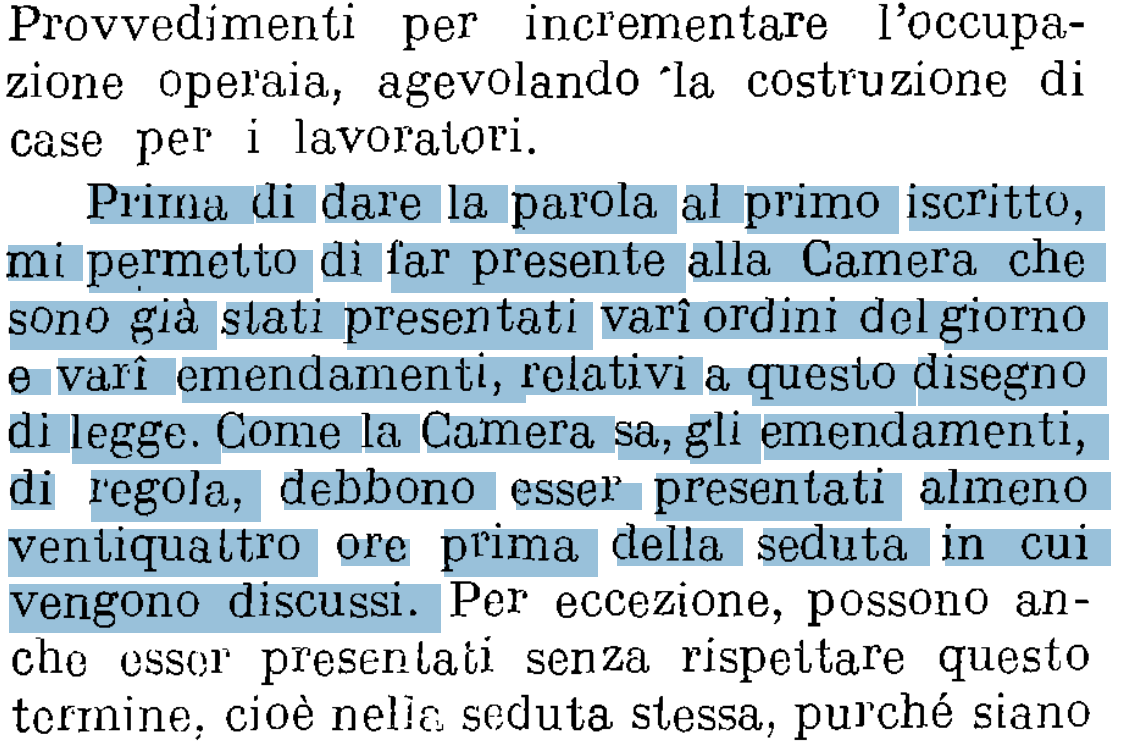
\includegraphics[width=\textwidth]{immagini/metodologia/ocr_ex.png}
\end{minipage} \hfill
\begin{minipage}{0.06\textwidth}
\Large$\rightarrow$
\end{minipage}
\begin{minipage}{0.5\textwidth}
\footnotesize	
Prima. di dare la parola al primo iscritto, \\
mi permetto di far presente alla Camera che \\
sono già stati presentati vari ordini del giorno \\
e var.1 emendamenti, relativi a questo disegno \\
di legge. Come la Camera sa, gli emendamenti, \\
di regola, debbono esser presentati alrneno \\
ventiquattro ore prima della seduta in cui \\
vengono discussi.
\end{minipage}
\caption{A sinistra un frammento di immagine contenente testo, a destra il testo digitalizzato estratto dal frammento di immagine.}
\label{fig:met_ocr_esempio}
}
\end{figure}

L'uso di sistemi OCR è particolarmente vantaggioso per l'archiviazione dei documenti. Infatti, l'estrazione del testo rende possibile eseguire sui documenti operazioni di ricerca e di reperimento informazioni. Si pensi a un'operazione basilare come la ricerca di tutti i documenti che contengono una determinata parola: un task dispendioso e manuale che è quasi istantaneo se si ha a disposizione il testo digitalizzato.
\paragraph{Errori}
I sistemi OCR presentano però alcuni problemi che possono influenzare negativamente le performance nel reperimento di informazioni \cite{impatto_ocr_1}\cite{impatto_ocr_2}. Si veda, ad esempio, il testo estratto in \autoref{fig:met_ocr_esempio}: seppur la maggior parte delle parole sono state riconosciute correttamente, è possibile notare alcuni errori. 
Generalmente la presenza di tali errori è dovuta a piccole imprecisioni nell'immagine iniziale: si pensi ad esempio un granello di polvere che può essere scambiato per un punto, o ad una \textit{"n"} battuta male che viene scambiata per la sequenza \textit{"ii"}.
Si possono distinguere le seguenti categorie di errore:
\begin{itemize}
\item \textbf{Word Error}. Aggiunta, rimozione o sostituzione di caratteri spuri all'interno di una parola. Questo tipo di errore si divide in due ulteriori sottocategorie:
	\begin{itemize}
	\item Non-word error (NW): la parola affetta da errore non è presente in un dato vocabolario. Un errore di questo tipo è la parola \textit{"gioia"} che diventa \textit{"g1o1a"}.
	\item Real-word error (RW): la parola affetta da errore è presente in un dato vocabolario, ma non è corretta nella frase in cui è inserita. Ad esempio, la frase \textit{"qualvolta i popoli ripongono la loro fiducia  nelle \ul{armi} e nella guerra"} può essere erroneamente interpretata come \textit{"qualvolta i popoli ripongono la loro fiducia  nelle \ul{ami} e nella guerra"}. "ami" è una parola presente nel vocabolario, ma non è corretta nel contesto della frase data.
	\end{itemize}
	
\item \textbf{Word Segmentation Error}. Si ha un errore di segmentazione quando aggiunte, rimozioni o sostituzioni di caratteri (incluso il carattere spazio) occorrono in maniera tale da dividere o unire parole. Sono considerati errori di segmentazione anche aggiunte di caratteri e segni di punteggiatura spuri all'interno del testo. Sono distinte le seguenti sottocategorie di errori di segmentazione:
	\begin{itemize}
	\item Space Splitting (SP), quando i caratteri di una parola o più parole adiacenti sono intervallati da spaziature. Ad esempio, si ha un errore di questo tipo nella frase \textit{"vostra presenza conferma l'\ul{attaccamento alla} cattedra di Pietro e la fedeltà al suo Magistero"} che viene letta come \textit{"vostra presenza conferma l'\ul{a t t a c c a m e n t o a l l a} cattedra di Pietro e la fedeltà al suo Magistero"}.
	\item Punctuation Splitting (DP), quando uno o più segni di punteggiatura dividono in più parti una parola. Ad esempio, data la parola \textit{"attaccamento"} si ha un errore DP quando essa viene interpretata come \textit{"at,tacc,amento"}.
	\item Punctuation Insertion (PS), quando uno o più segni di punteggiatura vengono aggiunti fra una parola e l'altra. Ad esempio, data la frase \textit{"Per secoli la Chiesa ha patrocinato artisti che hanno..."}, si hanno errori PS quando essa viene interpretata come \textit{"Per \ul{secoli'la} Chiesa \ul{ha.,patrocinato} artisti che hanno..."}.
	\end{itemize}
\end{itemize}

In \autoref{tab:met_esempio_errori} sono riportati ulteriori esempi degli errori appena elencati.

\begin{table}[H]
\centering
\begin{tabular}{cccc}
\textbf{Originale} & \textbf{OCR} & \textbf{Tipo} & \textbf{Errore} \\ \hline
dell'impresa & dell’iinpresa 	& NW & Sostituzione di "m" con "in" \\
interessano & iateressano 		& NW & Sostituzione di "n" con "a" \\
questo modo & questo nodo 		& RW & Sostituzione di "m" con "n" \\
l'ingordizia & I’ingordizia 	& RW & Sostituzione di "l" con "I" \\
produttrice & pro d u t t rice 	& SP & Parola spezzettata da spazi \\
azionisti & azi:misti 			& DP & Sostituzione con divisione della parola \\
vicinanze  del & vicinanze .del & PS & Introduzione di punteggiatura\\

\end{tabular}
\caption{Esempi di errori}
\label{tab:met_esempio_errori}
\end{table}

Se, come già detto, gli errori derivano spesso da piccoli difetti nell'immagine di partenza, è lecito aspettarsi una maggior quantità di errori da documenti più deteriorati o datati, come archivi storici. Per lo stesso motivo l'intensità degli errori può variare, a seconda delle condizioni in parti diverse di uno documento.

\paragraph{OCR Post-processing}
Una strategia spesso adottata per minimizzare il numero di errori è l'aggiunta di
una fase di post elaborazione (OCR post-processing) in seguito all'acquisizione
dei documenti tramite OCR. Lo scopo della fase di OCR post-processing è quello di correggere gli errori introdotti durante l'estrazione del testo dalle immagini. Una delle difficoltà in questa fase sta nel non introdurre nuovi errori nel testo. Si pensi ai seguenti casi:
\begin{itemize}
\item Il sistema prova a correggere una parola che non contiene errori. In questo caso, qualsiasi correzione risulterà in un nuovo errore. Una delle maggiori criticità nello sviluppare il sistema di correzione, infatti, sta nell'identificare correttamente gli errori all'interno del testo.
\item Il sistema identifica correttamente un errore, ma propone una correzione sbagliata. Si pensi al seguente esempio: \textit{"vesodvi"} viene erroneamente corretto in \textit{"vedovi"}. Tuttavia, la parola originale era \textit{"vescovi"}.
\end{itemize}

\ \\
La metodologia di correzione sviluppata è modellata come una pipeline che si compone di una serie di moduli ripetibili in sequenza. Ogni modulo è una funzione che si occupa di individuare e correggere una specifica categoria di errore.\\
La metodologia sviluppata si propone di correggere gli errori di tipo RW e SP.

\section{Architettura del sistema}
\label{sec:met_processo}

\subsection{Panoramica Generale}
\label{sec:met_panoramica}
Il sistema di correzione è articolato come una pipeline composta da uno o più moduli 	concatenati. Un modulo è una funzione il cui scopo è correggere una specifica tipologia di errore all'interno di una frase. Un modulo può essere formalmente definito come segue:
\begin{equation}
M: F \mapsto F\prime
\end{equation}
dove $F$ e $F\prime$ sono rispettivamente la frase originale e quella con delle correzioni apportate. \\
Sono stati definiti i seguenti moduli:
\begin{itemize}
\item \textbf{Modulo di correzione Token} ($M_{TK}$): individua e corregge tutti gli errori di tipo RW. \E\ discusso in dettaglio nella \autoref{sec:met_tok_correct}.
\item \textbf{Modulo di correzione Split} ($M_{SP}$): individua e corregge tutti gli errori di tipo SP. \E\ discusso in dettaglio nella \autoref{sec:met_mod_split}.
\end{itemize}

\begin{figure}[H]
\centering
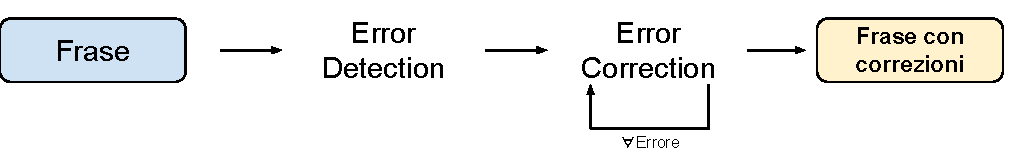
\includegraphics[width=\textwidth]{immagini/metodologia/modulo}
\caption{Schema del funzionamento di un modulo}
\label{fig:met_modulo}
\end{figure}

Come si può vedere in \autoref{fig:met_modulo}, il funzionamento di un modulo si compone delle fasi Error Detection (che da qui in poi sarà abbreviata con ED) ed Error Correction (che da qui in poi sarà abbreviata con EC). Durante la fase di ED vengono individuati gli errori presenti all'interno dalla frase da correggere: dato che moduli differenti correggono tipologie di errore differenti, ogni modulo applica una diversa strategia per individuare gli errori. Nella fase di EC vengono effettuate le correzioni degli errori individuati nella fase precedente.

\paragraph{Esempio} Si supponga di voler applicare alla seguente frase il modulo di correzione token:
\begin{center}
\textit{"\dashuline{Q o a l c h n} Papa \ul{nort} è compreso in questa comunità \ul{d1} morti \ul{gluriosi}"}
\end{center}
Il modulo di correzione token riconosce e corregge solo gli errori di tipo NW (Non-word error, sottolineati con linea continua), mentre ignora tutti gli errori di altro tipo (sottolineati con linea tratteggiata). L'output del modulo, supponendo di riuscire a correggere tutti gli errori, è il seguente:
\begin{center}
\textit{"\dashuline{Q o a l c h n} Papa non è compreso in questa comunità di morti gloriosi"}
\end{center}
\ \\
Data la definizione di modulo, è possibile definire una pipeline di correzione come una concatenazione di uno o più moduli. Più formalmente, una pipeline di correzione è definita come segue:
\begin{equation}
P: f_1 \circ f_2 \circ ... \circ f_n
\end{equation}
dove ogni $f_i$ è un modulo.
\begin{figure}[H]
\centering
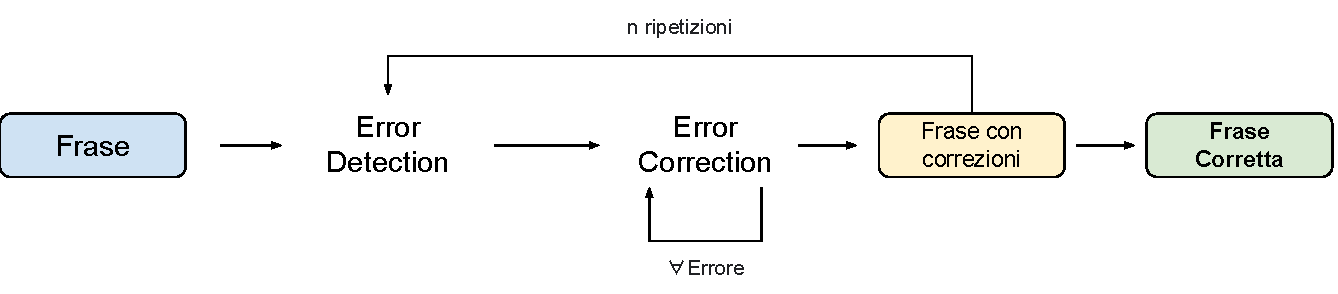
\includegraphics[width=\textwidth]{immagini/metodologia/generale}
\caption{Schema riassuntivo della pipeline di correzione}
\label{fig:met_generale}
\end{figure}

\paragraph{Esempio} Continuando l'esempio precedente, si supponga di concatenare un modulo $M_{SP}$ al precedente modulo $M_{TK}$. Il modulo riceve come input la frase con le correzioni apportate dal modulo precedente, e corregge tutti gli errori di tipo SP presenti nella frase (ovvero quelli con la sottolineatura tratteggiata):
\begin{center}
\textit{"Qualche Papa non è compreso in questa comunità di morti gloriosi"}
\end{center}



\ \\
All'interno della pipeline di correzione possono essere presenti più occorrenze di uno stesso modulo. In frasi con molti errori una sola applicazione di un dato modulo di correzione potrebbe non essere sufficiente per correggere tutti gli errori della propria tipologia. Per ragioni legate al funzionamento del BERT Masked Language Model che verranno meglio chiarite nelle prossime sottosezioni, infatti, ripetere un dato modulo più volte può aumentare tangibilmente le performance di correzione.

\begin{figure}[H]
\centering
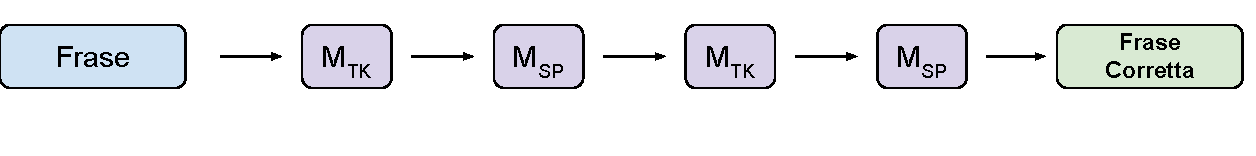
\includegraphics[width=\textwidth]{immagini/metodologia/pipeline_esempio}
\caption{Esempio di una possibile pipeline con più occorrenze di uno stesso modulo}
\label{fig:met_pipeline_esempio}
\end{figure}




\subsection{BERT Masked Language Modeling}
\label{sec:met_BERT_MLM}
La fase di error correction di entrambi i moduli implementati fa uso del BERT Masked Language Modeling (da qui in poi riferito come BERT MLM). Data una qualsiasi sequenza $S = [w_1,...,w_n]$ nella quale ogni $w_i$ è una parola, è possibile mascherare una sola parola $w_i$ con la stringa \textit{[MASK]}. Si ottiene così la sequenza con maschera $S\prime = [w_1,...,\text{[MASK]},...,w_n]$.\\
Dando in input $S\prime$ al modello BERT, esso associa ad ogni parola del proprio lessico la probabilità di corrispondere alla parola mascherata. Le prime n parole con la probabilità più alta sono dette candidati.
\E\ quindi formalizzata come segue la funzione del BERT MLM detta "mask-filling":
\begin{equation} \label{eq:met_BERT}
B: S\prime \rightarrow [c_1,...,c_n]
\end{equation}
dove ogni $c_i \in[c_1,...,c_n]$ è un candidato. 

\paragraph{Esempio} Data la frase 
\begin{center}
\textit{"che assistono ragazze in difficoltà, le persone \underline{soie} e abbandonate, gli ammalati e gli anziani."}
\end{center}
la parola \textit{"soie"} sottolineata è stata individuata come errore. \E\ quindi necessario mascherala, per dare la frase in input al modello BERT. La frase diventa dunque:
\begin{center}
\textit{"che assistono ragazze in difficoltà, le persone [MASK] e abbandonate, gli ammalati e gli anziani."}
\end{center}
BERT produce quindi una lista di candidati. Sono riportati i risultati impostando come soglia $n=5$. I candidati rappresentano le top-5 più probabili correzioni.
\begin{itemize}
\item \textit{"sole"} con probabilità 0.42
\item \textit{"anziane"} con probabilità 0.28
\item \textit{"povere"} con probabilità 0.08
\item \textit{"care"} con probabilità 0.03
\item \textit{"disabili"} con probabilità 0.01
\end{itemize}
\ \\
Bisogna sottolineare come la parola originale sia trasparente al modello BERT. Ciò significa che i candidati prodotti dal modello sono del tutto indipendenti dalla parola originale, e sono inferiti unicamente dal contesto derivato dal resto della frase.\\




\subsection{Modulo di correzione Token}
\label{sec:met_tok_correct}

\subsubsection{Error Detection}
\label{sec:met_tok_errdet}
Il modulo di correzione token ha lo scopo di individuare e correggere tutti gli errori di tipo NW.  L'individuazione degli errori è effettuata in modo automatico dopo
una pre-elaborazione (pre-processing) del testo. Il funzionamento di questa
fase può quindi essere suddiviso in due stadi:
\begin{enumerate}
\item \textbf{Sentence pre-processing}: la frase viene tokenizzata, ovvero viene divisa singole parole dette token. Questo stadio è implementato tramite la libreria NLTK\cite{nltk}.
\item \textbf{Error marking}: ogni token è analizzato singolarmente per determinare se contenga o meno un errore. Un token è considerato errato se sono vere le seguenti condizioni:
	\begin{itemize}
	\item Ha una lunghezza minima di 2 caratteri. Questa condizione è necessaria per evitare di introdurre nuovi errori correggendo inutilmente errori di tipo SP. Ad esempio, sarebbe deleterio provare a correggere le singole lettere di \textit{"Q u a l c h e"}. Ciò è dovuto al fatto che il modulo di correzione token è progettato per correggere singoli token: nell'esempio precedente, si tenterebbe quindi la correzione di tutte le sub-word che compongono il token. Per questo tipo di errori, è stato sviluppato di modulo di correzione Split (\autoref{sec:met_mod_split}).
	
	\item Dato un vocabolario di parole corrette, il token considerato non è presente in tale vocabolario. La ricerca nel vocabolario è eseguita in maniera case-insensitive. Tale approccio, seppur molto semplice, ha alcune criticità. Ad esempio, ogni parola non appartenente alla lingua italiana verrà segnalata come errore. \E\ quindi auspicabile disporre di un vocabolario che comprenda anche alcune parole straniere di uso comune.
	\end{itemize}
Un'eccezione a quest'ultima condizione è data da tutti i token che precedono un apostrofo. Questi token sono considerati corretti se almeno una fra tutte le combinazioni token + vocale è corretta. Si prenda ad esempio il token \textit{"dell"} non presente nel vocabolario, seguito dal token apostrofo. Vengono generate le 5 combinazioni token-vocale \textit{"della"},\textit{"delle"},\textit{"delli"},\textit{"dello"},\textit{"dellu"}. Siccome almeno una di queste è corretta, il token è considerato corretto.
\end{enumerate}

Il processo appena descritto è schematizzato in \autoref{fig:met_tok_errdet}. Tutti gli errori identificati sono poi corretti in sequenza dalla fase di error correction. 

\begin{figure}[H]
\centering
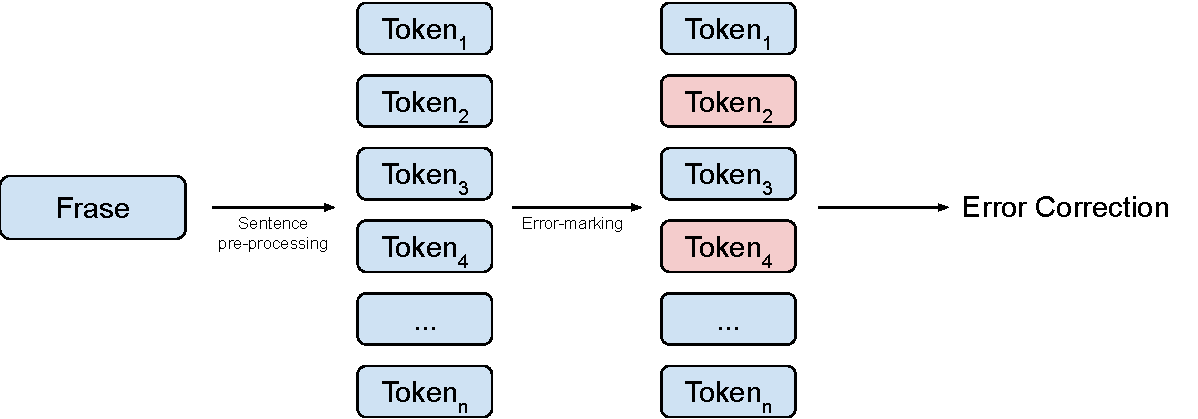
\includegraphics[width=\textwidth]{immagini/metodologia/error_detection}
\caption{Schema del processo di error detection}
\label{fig:met_tok_errdet}
\end{figure}

\subsubsection{Error Correction}
\label{sec:met_errcor}

La fase di error correction ha lo scopo di correggere gli errori individuati nella precedente fase. La fase di error correction è composta dai seguenti stadi:

\begin{enumerate}
\item Masking
\item Detokenization
\item Candidates generation and picking
\item Validation
\end{enumerate}

Ognuno di questi stadi è ripetuto per ognuno degli errori identificati durante la fase precedente.

\begin{figure}[H]
\centering
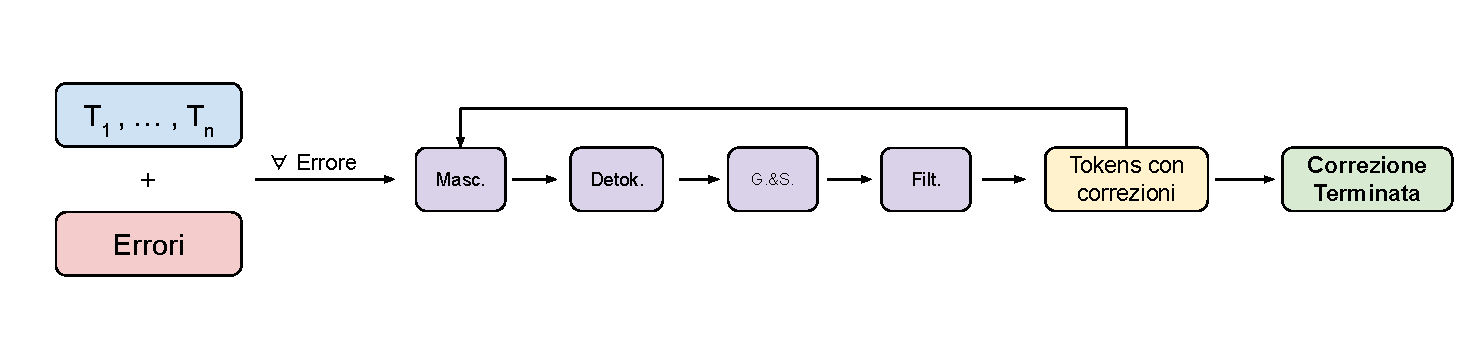
\includegraphics[width=\textwidth]{immagini/metodologia/tok_correction}
\caption{Schema della fase di error correction}
\label{fig:met_tok_correction}
\end{figure}



\paragraph{Masking}
Lo stadio di masking ha lo scopo di mascherare uno dei token errati individuati nella fase precedente. Si ricorda che, a causa del funzionamento del BERT MLM descritto nella \autoref{sec:met_BERT_MLM}, è possibile mascherare solo un token alla volta.\\
Data una sequenza di token $S = [t_1,...,t_n]$ e l'insieme $E = [t_i,t_j,...]\subseteq S$ dei token contenenti errore non ancora corretti, lo stadio di masking è descritto dalla seguente funzione:
\begin{equation}
M: S \rightarrow [t_1,...,\text{[MASK]},...,t_n] = S\prime
\end{equation}
dove \textit{[MASK]} sostituisce il primo token estratto dall'insieme $E$. Quanto descritto corrisponde al primo passaggio nella \autoref{fig:met_errgen}.


\paragraph{Detokenization}
Come spiegato nella \autoref{sec:met_BERT_MLM}, la funzione di mask-filling del BERT MLM richiede come input una sequenza intesa come frase, e non come insieme di token. \E\ quindi compito dello stadio di detokenization ricomporre una sequenza a partire dall'output dello stadio precedente. Lo stadio di detokenization è descritto dalla seguente funzione:
\begin{equation}
D: [t_1,...,\text{[MASK]},...,t_n] \rightarrow F_{mask}
\end{equation}
dove $F_{mask}$ è una frase contente una maschera.

\paragraph{Candidates generation and picking}
Lo stadio di candidates generation and picking sfrutta il BERT MLM per generare dei candidati per la correzione, e sfrutta un'euristica per determinare il candidato con la maggior probabilità di essere corretto (da qui in poi riferito come soluzione). Più precisamente, la generazione dei candidati avviene tramite la funzione di mask-filling descritta nell'\autoref{eq:met_BERT} (\autoref{sec:met_BERT_MLM}). La fattibilità di applicare tale approccio per la generazione di candidati per la correzione è dimostrata in \cite{OCRMaskFilling}. Nel paper appena citato si riporta come, usando una combinazione di BERT e FastText, la giusta correzione da applicare sia presente fra i candidati prodotti con una probabilità del 70\%. Risultati comparabili sono stati ottenuti con una metodologia simile dai test illustrati nella \autoref{sec:analisi}.\\
Lo step di generazione dei candidati è formalizzato come segue:
\begin{equation}
G: F_{mask} \rightarrow [c_1,...,c_n]= C
\end{equation}
dove ogni $c_i$ è un candidato.\\
L'euristica per la scelta della soluzione sceglie il candidato con la più bassa distanza di Levenshtein dal token mascherato. Più formalmente, chiamando $m$ il token mascherato, la soluzione $s$ è definita come segue:
\begin{equation}
s = \operatorname*{argmin}_{c_i \in C} d_{lev}(c_i,m)
\end{equation}
In caso uno o più candidati abbiano la stessa distanza dal token mascherato, viene scelto quello con la maggior probabilità prodotta da BERT. Questa euristica, seppur molto semplice, è decisamente efficace, come dimostrato dall'analisi nella \autoref{sec:ana_cor}.

\begin{figure}[H]
\centering
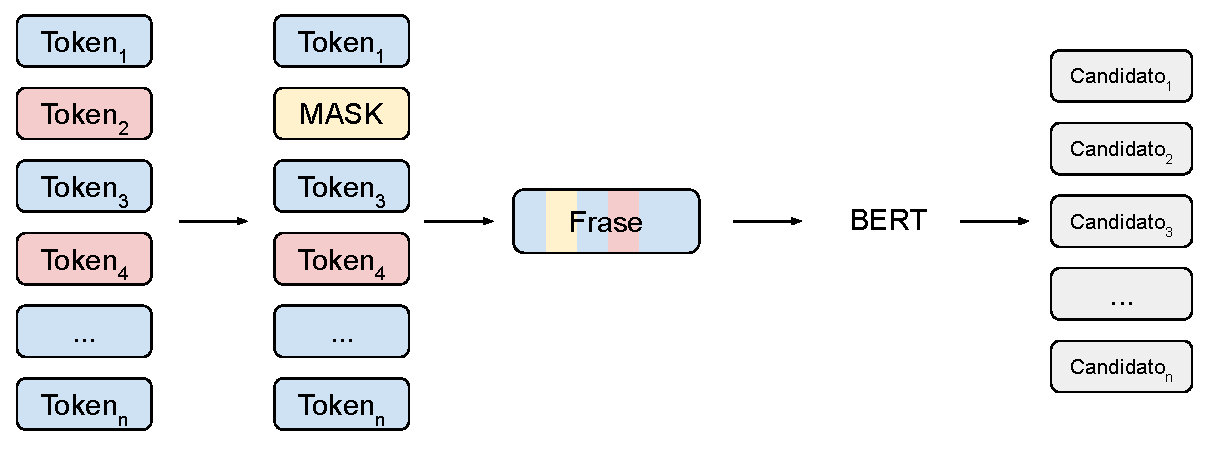
\includegraphics[width=\textwidth]{immagini/metodologia/generazione_candidati}
\caption{Schema del processo di generazione e scelta dei candidati}
\label{fig:met_errgen}
\end{figure}

\paragraph{Validation}
Può accadere che la soluzione non sia una correzione adatta: si pensi ai seguenti casi:
\begin{enumerate}
\item L'error detection contrassegna un token corretto come errore. In questo caso, ogni tentativo di correzione introdurrebbe nuovi errori all'interno del testo.
\item BERT non produce la giusta correzione fra i candidati. Anche in questo caso, qualunque sia il candidato scelto, il sistema di correzione andrebbe a introdurre nuovi errori all'interno del testo.
\end{enumerate}

\E\ introdotta quindi un'ulteriore fase di validation, con lo scopo di valutare se la soluzione prodotta possa o meno rappresentare una correzione valida. La validazione è implementata tramite un'euristica che valuta se la soluzione trovata è troppo lontana (in termini di distanza di Levenshtein) dal token mascherato. Chiamando $l$ la lunghezza in caratteri del token mascherato, e $d$ la distanza di Levenshtein fra il token mascherato e la soluzione trovata, la soluzione è valida se:
\begin{itemize}
\item $l > 10 \wedge d < 5$ 
\item $l > 5 \wedge d < 4$ 
\item $l \leqslant 5 \wedge d < 3$ 
\end{itemize}
Se la validazione scarta la soluzione trovata il sistema ignora la correzione. Al contrario, se la validazione ritorna esito positivo, la correzione viene sostituita al token mascherato. Quanto appena descritto è rappresentato in \autoref{fig:met_pick}.

\begin{figure}[H]
\centering
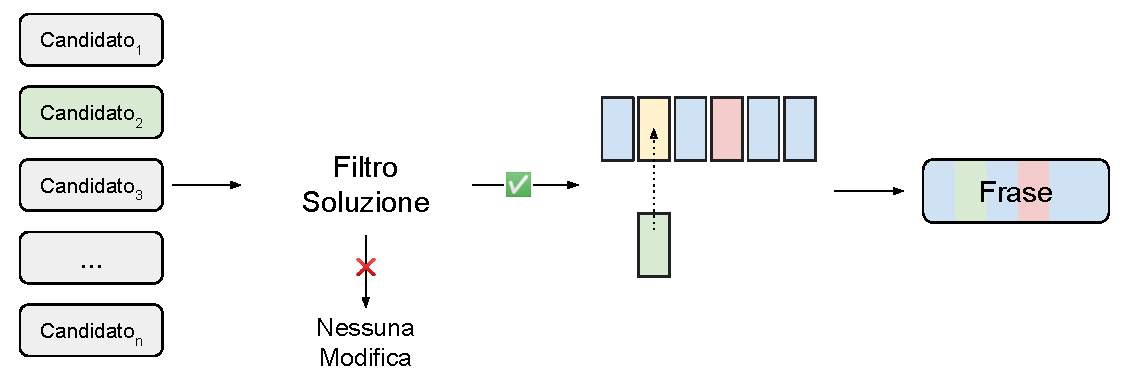
\includegraphics[width=\textwidth]{immagini/metodologia/scelta_candidati}
\caption{Schema del processo di scelta dei candidati}
\label{fig:met_pick}
\end{figure}
Il processo appena descritto si ripete per ogni errore contrassegnato durante la fase di error detection. Una volta completata la correzione dell'ultimo token errato, la fase di error correction può dirsi conclusa.

\subsubsection{Ripetizione}
In frasi contenenti molti errori, è possibile che una sola applicazione del modulo di correzione token non basti correggere tutti i non-word errors.\\
Ciò è dovuto al funzionamento di BERT, che usa il contesto a destra e sinistra della maschera per produrre i candidati di correzione. Se questo contesto è sporcato da molti errori, è più probabile che BERT non sia in grado di produrre una soluzione adeguata. \E\ quindi possibile che dopo l'applicazione di questo o altri moduli, e la conseguente correzione di alcuni errori, sia possibile ottenere migliori risultati sulle correzioni precedentemente non riuscite.\\
Questo approccio comporta però uno svantaggio: se la prima o una della prime correzioni sono sbagliate, il rischio è quello di introdurre rumore anche nelle correzioni successive.

\subsection{Modulo di correzione Split}
\label{sec:met_mod_split}

\subsubsection{Error detection}
\label{sec:met_split_errdet}
Il modulo di correzione Split corregge tutti gli errori di tipo SP.\\
La fase di error detection si compone di tre stadi:
\begin{enumerate}
\item \textbf{Sequences marking}: data una frase contenente errori di tipo SP, sono delimitati i punti di inizio e terminazione delle sequenze contenenti errori. L'individuazione di tali sequenze è eseguita tramite la seguente espressione regolare:
\begin{lstlisting}[language=Python]
r'(?:\s|^)(\w(?:\W?\s\w{1,2}){3,})(?:\W|\s|$)'
\end{lstlisting}
La precedente espressione regolare intercetta tutte le sequenze di almeno tre gruppi di caratteri alfanumerici con lunghezza massima due intervallati da spazi e/o caratteri non alfanumerici. Per maggiore chiarezza, in \autoref{table:met_split_esempi} sono riportati alcuni esempi di sequenze riconosciute.

\item \textbf{Punctuation filtering}: all'interno delle sequenze vengono rimossi tutti i caratteri non alfanumerici o spaziature. Ciò serve e rimuovere eventuali segni di punteggiatura spuri che possono diminuire l'efficacia delle seguenti fasi.

\item \textbf{Error validation:} non tutte le sequenze riconosciute dall'espressione regolare sono degli errori. Si pensi ad esempio ad una serie di preposizioni o congiunzioni, come il quarto esempio in \autoref{table:met_split_esempi}. Si usa quindi un'euristica per scartare le sequenze che si ritiene non contengano errori. Sono considerati errori tutte le sequenze nelle quali il numero di gruppi di 2 caratteri è minore del numero di gruppi di 1 carattere.

\end{enumerate}


\begin{table}[H]
	\centering
	\begin{tabular}{cccc}
	\textbf{\#} & \textbf{Frase} & \textbf{Sequenza} & \textbf{Errore} \\ \hline
	
	1 &\textit{"d i l e t t i membri, della ..."}	&	\textit{d i l e t t i}	&	Sì \\
	2 &\textit{"guidato d ui l l a fede"}			& 	\textit{d ui l l a}		&	Sì \\
	3 &\textit{"... altro tipo di u n i o, n e."}	&	\textit{u n i o, n e}	&	Sì \\
	4 &\textit{"in me e io in te, siano anch..."}	&	\textit{in me e io in te}&	No \\
	5 &\textit{"...dopo qu al ch e esitazione..."}	&	\textit{qu al ch e}&	Sì\\
	6 &\textit{"...dopo q u al che esitazione..."}	&	\textit{q u al}&	Sì\\
	7 &\textit{"...dopo qu al che esitazione..."}	&	/ &	/\\
	\end{tabular}
	\caption{Esempi di sequenze riconosciute}
	\label{table:met_split_esempi}
\end{table}
L'approccio di error correction appena esposto presenta però alcune limitazioni. Se uno dei gruppi della parola divisa contiene più di tre caratteri alfanumerici, la sequenza prodotta può:
\begin{itemize}
\item Non essere riconosciuta. \E\ il caso dell'esempio 7 nella \autoref{table:met_split_esempi}. In questo caso, il gruppo \textit{"che"} non è catturato dall'espressione regolare. Ciò comporta che il numero di gruppi di caratteri sia troppo basso per essere riconosciuto dall'espressione regolare.
\item Essere riconosciuta parzialmente.  \E\ il caso dell'esempio 6 nella \autoref{table:met_split_esempi}. In questo caso, il gruppo \textit{"che"} non è catturato dall'espressione regolare. Ciò comporta che venga catturata la sequenza \textit{"q u a l"}, che verrà corretta, introducendo possibilmente un errore. Il gruppo \textit{"che"}, invece, viene erroneamente considerato corretto.
\end{itemize}
\ \\
Data quindi una frase $f \in F$ contenente errori di segmentazione, dove $F$ è l'insieme di tutte le frasi, la fase di error detection è formalizzata come segue:
\begin{equation}
\textit{ED}_{split}: F \rightarrow L_{seq}
\end{equation}
dove ogni $l_{seq} \in L_{seq}$ è un insieme di tuple $[(s_1,b_1,e_1),...,(s_n,b_n,e_n)]$ nel quale ogni tupla corrisponde ad un errore individuato e validato. Ogni tupla è composta come segue:
\begin{itemize}
\item $s_i$ è la sequenza filtrata contenente l'errore
\item $b_i$ è il punto di inizio in $f$ della sequenza
\item $e_i$ è il punto di fine in $f$ delle sequenze
\end{itemize}

%\begin{figure}[H]
%\centering
%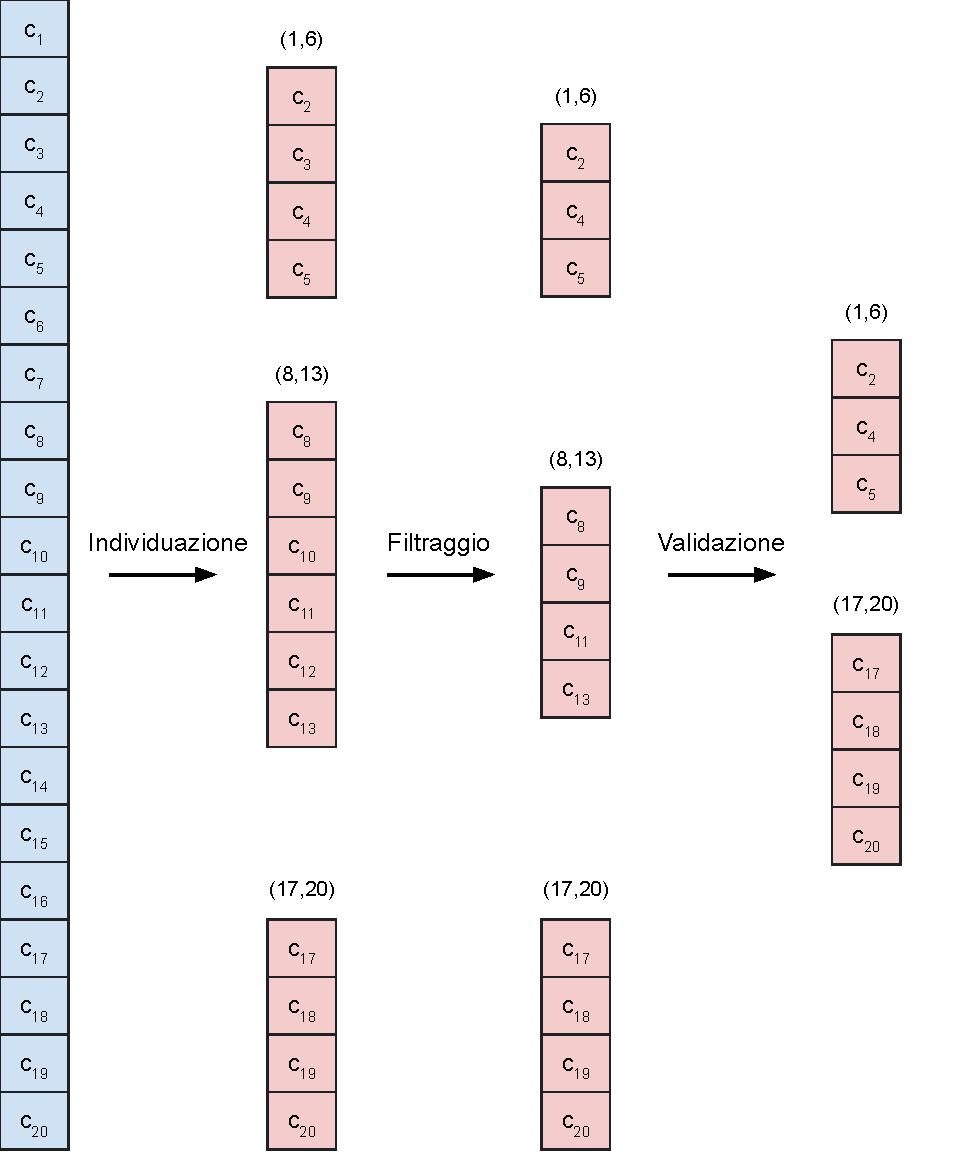
\includegraphics[width=\textwidth]{immagini/metodologia/split_error_detection}
%\caption{Schema del processo di error detection. Nell'immagine, ogni $c_i$ è un carattere}
%\label{fig:met_split_errdet}
%\end{figure}

\paragraph{Esempio}
Data la frase:
\begin{center}
\textit{coinvolsero ogni uomo \ul{e o' g n i} donna, \ul{p r o c u r a n d o}.}
\end{center}


\begin{table}[H]
\centering
\tabcolsep=0.16cm
\begin{tabular}{|c|c|c|c|c|c|c|c|c|c|c|c|c|c|c|c|c|c|c|c|c|c|c|c|c|c|c|c|c|c|}
\hline
0&1&2&3&4&5&6&7&8&9&10&11&12&13&14&15&16&17&18&19\\
\hline
c&o&i&n&v&o&l&s&e&r&o& &o&g&n&i& &u&o&m\\
\hline
\end{tabular}
\end{table}
\begin{table}[H]
\centering
\tabcolsep=0.11cm
\begin{tabular}{|c|c|c|c|c|c|c|c|c|c|c|c|c|c|c|c|c|c|c|c|c|c|c|c|c|c|c|c|c|c|}
\hline
20&21&22&23&24&25&26&27&28&29&30&31&32&33&34&35&36&37&38&39\\
\hline
o& &e& &o&'& &g& &n& &i& &d&o&n&n&a&,&\\
\hline
\end{tabular}
\end{table}
\begin{table}[H]
\centering
\tabcolsep=0.11cm
\begin{tabular}{|c|c|c|c|c|c|c|c|c|c|c|c|c|c|c|c|c|c|c|c|c|c|c|c|c|c|c|c|c|c|}
\hline
40&41&42&43&44&45&46&47&48&49&50&51&52&53&54&55&56&57&58&59\\
\hline
p& &r& &o& &c& &u& &r& &a& &n& &d& &o&.\\
\hline
\end{tabular}
\caption{Caratteri e indici della frase di esempio}
\end{table}




si procede con lo stadio di sequences marking. Le sequenze individuate sono quelle sottolineate nella frase data. Sono riportate di seguito insieme alla loro posizione di inizio e di fine.
\begin{table}[H]
\centering
\begin{tabular}{cccc}
\#&\textbf{Sequenza} & \textbf{Pos.Inizio} & \textbf{Pos.Fine}\\ \hline
1&\textit{"e o' g n i"}&22& 32\\
2&\textit{"p r o c u r a n d o"}& 40& 59\\
\end{tabular}
\end{table}

Si procede quindi con lo stadio di punctuation filtering:
\begin{table}[H]
\centering
\begin{tabular}{cccc}
\#&\textbf{Sequenza} & \textbf{Pos.Inizio} & \textbf{Pos.Fine}\\ \hline
1&\textit{"e o g n i"}&22& 32\\
2&\textit{"p r o c u r a n d o"}& 40& 59\\
\end{tabular}
\end{table}
Si noti come nella prima sequenza è stato cancellato un apostrofo, ma le posizioni di inizio e fine rimangono le stesse, in quanto demarcano l'inizio e la fine della sequenza nella frase originale. Lo stadio di error validation in questo caso non scarta alcuna soluzione: in entrambe le sequenze, infatti, il numero di gruppi di 1 carattere è maggiore del numero di gruppi di 2 caratteri.

\subsubsection{Error correction}
\label{sec:met_split_errcor}
La fase di Error Correction mira a correggere gli errori individuati nella fase precedente. Più formalmente è definita come:
\begin{equation}
EC_{split}: (F,L_{seq}) \rightarrow F_{corr}
\end{equation}
dove $F_{corr}$ è la frase con le correzioni apportate.\\
La fase di Error Correction si compone dei seguenti stadi:
\begin{enumerate}
\item \textbf{Compression:} per ogni sequenza $s_i$ individuata da correggere, si rimuovono gli spazi bianchi, in modo da ottenere un'unica parola continua detta $s\prime_i$.
\item \textbf{Vocabulary correction}: se una sequenza $s\prime_i$ è presente nel vocabolario, allora $s\prime_i$ viene inserita nella frase al posto della sequenza contenente l'errore.
\item \textbf{BERT correction:} si fa uso del BERT MLM per trovare una correzione, in modo simile a quanto fatto nel modulo di correzione token. A seconda della tipologia dell' errore sono applicabili due strategie di correzione.
		\begin{itemize}
		\item Con sottrazione		
		\item Con rimpiazzo		
		\end{itemize}
\end{enumerate}

Ognuno degli stadi appena descritti è applicato in sequenza ad ogni singola tupla prodotta dalla fase precedente.

\paragraph{Funzione di sostituzione}
Viene introdotta una funzione detta funzione di sostituzione. Data una frase $f \in F$, una sequenza $s \in S$, un valore di inizio $b \in I$ e un valore di fine $e \in E$, la funzione è definita come:
\begin{equation}
\textit{Sos}: (F,S,I,E) \rightarrow F\prime
\end{equation}
dove $F\prime$ è la frase $F$ in cui tutti i caratteri fra $b$ ed $e$ sono stati sostituiti da $s$.\\
Alternativamente, definendo come $T$ la tupla $(s,b,e)$ è possibile scrivere la funzione anche come segue:
\begin{equation}
\textit{Sos}: (F,T) \rightarrow F\prime
\end{equation}
Ad esempio, data la frase $f_{es}$:
\begin{center}
\textit{Onorando una trod1z1one plurisecolare}
\end{center}
e la tupla $t_{es}$ (\textit{"tradizione"},14,25), si ha che:
\begin{equation}
\textit{Sos}(f_{es},t_{es}) = \textit{Onorando una tradizione plurisecolare}
\end{equation}


\paragraph{Compression}
Lo stadio di compression rimuove gli spazi da ogni sequenza $s$ individuata come errore. Più formalmente, data una tupla $(s,b,e) \in T$ , lo stadio di compression è definito come segue:
\begin{equation}
\textit{Comp}: T \rightarrow T\prime
\end{equation}
dove $T\prime$ è l'insieme di tutte le tuple $(s\prime,b,e)$ in cui $s\prime$ è la sequenza $s$ senza spaziature. Riprendendo l'esempio proposto nella fase di error detection, le tuple prodotte diventano rispettivamente:
\begin{table}[H]
\centering
\begin{tabular}{cccc}
\#&\textbf{Sequenza} & \textbf{Pos.Inizio} & \textbf{Pos.Fine}\\ \hline
1&\textit{"eogni"}&22& 32\\
2&\textit{"procurando"}& 40& 59\\
\end{tabular}
\end{table}

\paragraph{Vocabulary correction}
Date le tuple prodotte dallo stadio precedente, lo stadio di vocabulary correction applica una correzione per tutte le tuple la cui sequenza corrisponde ad una parola presente nel vocabolario. \\
Data quindi la frase $F$ contenente errori di segmentazione e una tupla $(s\prime,b,e)$ detta $t_{corr}$ che rispetta la condizione enunciata precedentemente, la frase con la correzione applicata $F_{corr}$ si ottiene come segue:
\begin{equation}
F_{corr} = \textit{Sos}(F,t_{corr})
\end{equation}
Se la tupla che si sta trattando può essere utilizzata per una correzione con vocabolario, la correzione si arresta in questo stadio. Altrimenti, si procede allo stadio di BERT correction.\\
Continuando l'esempio predente, si nota come la seconda tupla contenga la sequenza "procurando" che è una parola all'interno del vocabolario. Ricordando la frase originale
\begin{center}
\textit{coinvolsero ogni uomo e o' g n i donna, p r o c u r a n d o.}
\end{center}
detta $F_{ex}$, e la tupla $t_2$ (\textit{"procurando"}, 40, 59), la correzione si applica come segue:
\begin{equation}
F_{corr} = \textit{Sos}(F_{ex},t_{2})
\end{equation}
Il risulta è la frase $F_{corr}$:
\begin{center}
\textit{coinvolsero ogni uomo e o' g n i donna, procurando.}
\end{center}


\paragraph{BERT correction}
Per tutte le tuple per le quali non è stato possibile applicare una correzione con vocabolario, si passa allo stadio di BERT correction. Il primo step di questo stadio consiste nel mascheramento della sequenza errata nella frase originale. Data una tupla $(s\prime,b,e)$ prodotta dallo stadio di compressione e una frase $F$, si ottiene la frase mascherata $F_{mask}$ come segue:
\begin{equation}
F_{mask} = \textit{Sos}(F,\textit{[MASK]},b,e)
\end{equation}
A questo punto si sfrutta il BERT MLM per produrre un candidato per la correzione. Il processo è analogo alla fase di generazione e scelta dei candidati del modulo di correzione token nella \autoref{sec:met_errcor}, per cui si rimanda il lettore al paragrafo che ne spiega il funzionamento.\\
Una volta prodotto il candidato per la correzione, detto $c_{corr}$, è possibile applicare una correzione per sottrazione o per rimpiazzo.


\paragraph{Correzione con sottrazione}
Si applica in caso $c_{corr}$ coincida con la fine o l'inizio della sequenza compressa $s\prime$. Questo è il caso in cui la sequenza riconosciuta come errore di spezzettamento con spazi comprende due parole. Pertanto, se $c_{corr}$ corrisponde all'inizio di $s\prime$, si ottengono le due stringhe $\textit{sub}_1$ e $\textit{sub}_2$ come segue:
\begin{equation}
\textit{sub}_1,\textit{sub}_2 = c_{corr}, s\prime -c_{corr}
\end{equation}
Se invece $c_{corr}$ corrisponde alla fine di $s\prime$, le stringhe $\textit{sub}_1$ e $\textit{sub}_2$ si ottengono  come segue:
\begin{equation}
\textit{sub}_1,\textit{sub}_2 = s\prime -c_{corr},c_{corr},
\end{equation}
Data quindi la frase $F$ contenente errori di segmentazione, la tupla $(s\prime,b,e)$ e le stringhe $\textit{sub}_1,\textit{sub}_2$, la frase con la correzione applicata $F_{corr}$ si ottiene come segue:
\begin{equation}
F_{corr} = \textit{Sos}(F, \textit{sub}_1 + "\ " + \textit{sub}_2  ,b,e)
\end{equation}
La correzione con sottrazione corregge i casi in cui la sequenza contenente errore è formata da due parole. Può accadere che la stringa $s\prime -c_{corr}$ non rappresenti una parola corretta, ovvero potrebbe non essere presente nel vocabolario. Non sono previsti controlli e contromisure ad hoc per tale eventualità: la correzione di eventuali errori di questo tipo è delegata ai moduli di correzione token che possono essere inseriti a valle nella pipeline.\\
Si consideri ora l'esempio portato avanti negli stadi precedenti: data la tupla $t_2$ (\textit{"eogni"}, 22, 32) e la frase $F_{ex}$
\begin{center}
\textit{coinvolsero ogni uomo e o' g n i donna, p r o c u r a n d o.}
\end{center}
si ottiene come la frase $F_{mask}$ applicando la funzione di sostituzione:
\begin{equation}
F_{mask} = \textit{Sos}(F_{ex},\textit{[MASK]},22,32)
\end{equation}
Si ottiene dunque la frase
\begin{center}
\textit{coinvolsero ogni uomo [MASK] donna, p r o c u r a n d o.}
\end{center}
Sfruttando il BERT MLM si ottiene il candidato $c_{corr}$ "ogni". Il candidato corrisponde alla fine di $s\prime$, pertanto si ottengono $\textit{sub}_1,\textit{sub}_2 = \textit{e}, \textit{ogni}$. Si applica quindi la funzione di sostituzione:
\begin{equation}
F_{corr} = \textit{Sos}(F_{ex}, \textit{e} + "\ " + \textit{ogni} ,22,32)
\end{equation}
La frase corretta $F_{corr}$ è quindi: 
\begin{center}
\textit{coinvolsero ogni uomo e ogni donna, p r o c u r a n d o.}
\end{center}

\paragraph{Correzione con rimpiazzo}
Si applica in caso $c_{corr}$ non coincida con la fine o l'inizio della sequenza compressa $s\prime$. Questo step utilizza un'euristica per validare la correzione prodotta dal BERT MLM. La soluzione prodotta da BERT è valutata ammissibile se e solo se $d_{lev}(s\prime,c_{corr}) \leqslant 4$.\\
In caso la soluzione sia ammissibile, la correzione è applicata tramite la funzione di sostituzione:
\begin{equation}
F_{corr} = \textit{Sos}(F,c_{corr},b,r)
\end{equation}
In caso la soluzione non sia ammissibile, la correzione si arresta senza apportare correzioni.




















\chapter{Implementazione, Test e Risultati}
\label{sec:test}

\chapter{Analisi dell'errore}
\label{sec:analisi}






\bibliographystyle{unsrt}
\bibliography{../bibliografia}


\end{document}


 
